This section describes the history of the sequencer changes since Run 7. Run 7 results were obtained with the v30 sequencer. The changes made for v30 are documented in Section 5.2 of \cite{SITCOMTN-148}. Since Run 7 was concluded, additional optimization targets were defined:
\begin{itemize}
    \item Eliminating long-range correlations 
    \item Reducing readout noise by switching to 3\,s readout timing
\end{itemize}

Our testing of the resulting optimizations was simplified owing to schedule pressure to begin the Science Verification survey.


\subsubsection{Long-range correlations}
%%
%% describe what the long range correlation etc...
The measurement of brighter-fatter coefficients reported in \cite{SITCOMTN-148} had already shown an anomalously high value of the \(a_{00}\) coefficient for one specific e2v sensor: R23\_S02 (see Figure 34 in that note). 
This measurement is derived from fits over the variance and spatial covariance curves versus the flux. The curves for the channels in that particular sensor were in fact affected by an excess of variance, which affected not only the noise measurement in bias frames, but also introduced an extra flux-dependent component in the variance. This degraded the gain measurements from the PTC (using \(C_{00}/\mu\)).
This issue also manifested as a flux-dependent covariance between amplifiers in the same sensor, and as an excess in the correlation with the next pixel in the serial direction (\(a_{10}\)). One way to detect this issue in a systematic manner is to compute the slopes of the covariances between channels versus the flux, and average them over all channels in the sensor (as done in Figure~\ref{fig:covariance-RGn20}). Using this metric, other sensors were found to exhibit a similar issue, but to a smaller degree (same Figure, left plot). 
Other related metrics (noise correlation between channels, correlations between channels) also pointed to the same sensors.

\begin{figure}[ht]
\begin{centering}
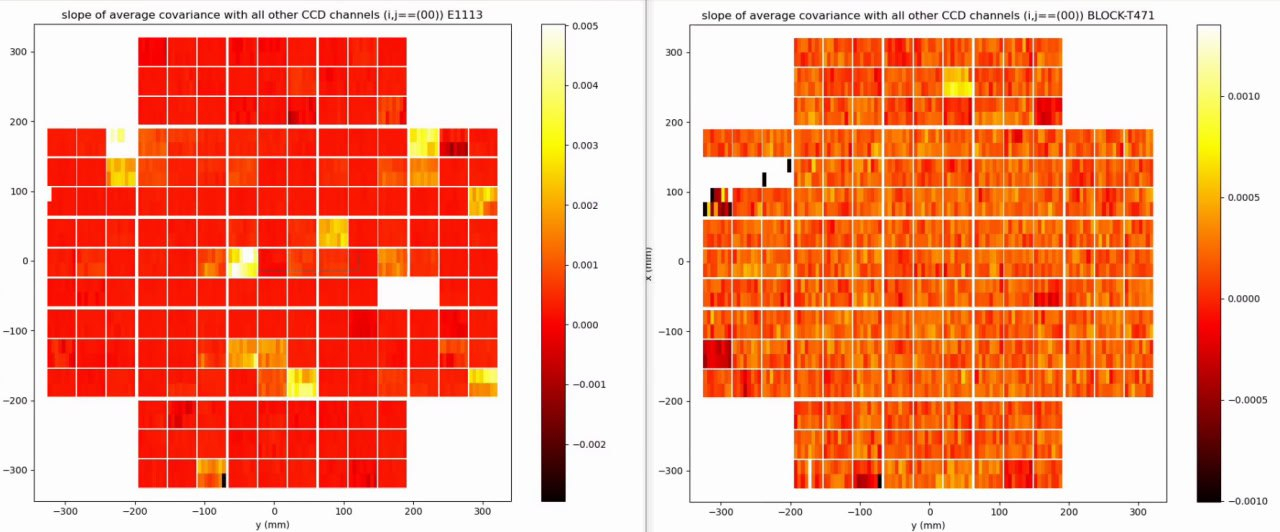
\includegraphics[width=0.9\textwidth]{sequencer/slopes-cov-before-after.jpg}
\caption{Averages of the slopes of the covariances between channels, for each sensor. Left: during test Run 7. Right: on sky, with the modified 'RGn20' readout sequence.}
\label{fig:covariance-RGn20}
\end{centering}
\end{figure}

Since the issue affected some sensors uniformly, and exhibited flux dependency, investigations focused on the CCD readout clocks, and in particular on the pixel reset clock (RG). 
To explain a potential variation from sensor to sensor, it should be noted that while the REB FPGA drives all three sensors with the same readout sequence, the actual clocks are generated on a per-sensor basis. 
While the jitter of the FPGA timing signal is in the range of 100\,ps, the jitter in the chain that translates that signal into a clock can be 1-3\,ns. In addition, the RG clock is faster than the serial clocks, due to a lower capacitive load.

For sensors like R23\_S02, plots acquired in scan mode at the raft level showed a strong variability (dispersion over consecutive scans) in the timing of the clock transitions around the time that the pixel reset (RG) clock was lowered. 
In the e2v sequence for pixel readout, this drop of the RG clock was timed simultaneously with the drop of the S2 clock (which transfers charges to the S3 phase, in preparation for transfer to the readout node). 
The same scans also showed a much stronger variability in the level of the signal after the pixel reset, up to 1000 electrons instead of the expected 50-100 electrons from \(kTC\) noise. Even with the Dual Slope Integration that is performed in the CCD readout chain, such high variability would explain an extra component in the noise.
 
We then tested a series of modifications to the timing of the readout sequence. 
In a sensor that did not exhibit the extra covariance with the nominal timing, we were able to induce it by triggering the S2 clock drop 10\,ns before the RG drop.
Conversely, tests on sensors that exhibited the issue showed that delaying the S2 drop by an increment of 10 or 20\,ns after the RG drop removed the issue (Figure~\ref{fig:covariance-RGn20}, on the right). 
A 20\,ns delay was selected as the safer option, and added to the e2v readout sequence (tagged as v30\_RGn20, then adopted as v31). 
A similar modification was tested on ITL sensors, which had no effect on sensors that exhibited correlated noise.


v32 has a stuff related to idle clear, no functional changes in other parts
v33 is reordered in a one-part sequencer in timing. Whether inserting a 20ns RG before (as BufferRGp) or after the BufferS+TimeS (as BufferRGn) time slice. No change in the total timing.

\subsubsection{3\,s sequencer file development}
The observing strategy has evolved from two snaps of 15\,s exposures to a single 30\,s exposure per visit.  By eliminating the intermediate readout, the overall timing budget is relaxed: one full readout cycle no longer needs to be performed every 15\,s.  
This reduction frees up readout time that can be reallocated to decrease readout noise.  Consequently, the development of a 3\,s sequencer (instead of the existing 2\,s) was initiated to take advantage of this additional margin.

%%
%% Timing chart
%%
We examined the time slices in the sequencer files and identified four key parameters for optimization:

\begin{itemize}
\item ISO1: Time for ASPIC clamp/reset to start of the first integration to measure the baseline (Ramp Down; RD)
\item ISO2: Time between S3 down and start of ASPIC Ramp Up (RU)
\item RampTime: Ithe integration time of a pixel read.
\item TimeP: Unit element of the Parallel Transfer (parallel timing).
\item BufferP: Time period before each parallel transfer starts. 
\end{itemize}

Previous studies \citep{10.1117/12.3019117,2024SPIE13103E..21S} examined how variations in ISO1, ISO2 and RampTime affect readout noise; they also demonstrated that altering Parallel Transfer (TimeP) can increase full-well capacity. ISO2 is additionally known to influence crosstalk.
For the v30 firmware, BufferP is set to 3360\,ns, raising the question of whether the entire parallel clocking should be shifted forward as in the original vendor sequence. In fact this change 
Because extending ISO1 degraded performance on some e2v sensors, our investigation was confined to the following scenarios: 
\begin{enumerate}
    \item \textbf{Longer integration time per pixel (3s-v0 RT)} – RampTime increase= from 380 to 620\,ns (factor 1.6)
    \item \textbf{Extended ISO2 duration (3s-v0 ISO2)} – lengthen the readout interval for each row.
    \item \textbf{Longer parallel transfer timing (3s-v0 Parallel)} – Allow more time for charge transfer between columns.
\end{enumerate}
Design constraints emphasized minimal deviation from the baseline sequencer, preserving parameters that had been previously tuned. 

\begin{tikzpicture}[
    % Define the distance between nodes
    node distance=1.5cm,
    % Define the common style for boxes
    box/.style={rectangle, draw, minimum width=2.5cm, minimum height=0.7cm, align=center}
]
    
    % Node placement
    \node (iso2) [box] {ISO2};
    % The right=2.5cm is the distance from edge to edge
    \node (3s_v0) [box, right=2.5cm of iso2] {3s-v0 RT};
    \node (parallel) [box, right=2.5cm of 3s_v0] {Parallel};
    % Vertical nodes
    \node (2s_v33) [box, above=2.5cm of 3s_v0] {2s-v33};
    \node (2s_v30) [box, above=2.5cm of 2s_v33] {2s-v30};
    \node (3s_v1)  [box, below=2cm of iso2] {3s-v1};
    \node (3s_v2)  [box, below=2cm of 3s_v1] {3s-v2};
    
    % Draw arrows (edges) and add labels
    
    % 0. 3s-v0 RT -> 2s-v33 (Vertical Up)
    % Use midway, right to place the label to the right of the center of the line, and text width for wrapping.
    \draw[->] (2s_v30.south) -- (2s_v33.north)
        node[midway, right, align=left, text width=5cm] 
        {(long range correlation and guider functionality)};        % 1. 3s-v0 RT -> 2s-v33 (Vertical Up)
        
    % Use midway, right to place the label to the right of the center of the line, and text width for wrapping.
    \draw[->] (2s_v33.south) -- (3s_v0.north)
        node[midway, right, align=left, text width=5cm] 
        {(increased RT / change in Buffer P)};    
        
    % 2. ISO2 -> 3s-v0 RT (Horizontal)
    \draw[->] (iso2) -- 
        node[midway, above] {(increase ISO2)} 
        (3s_v0);
    
    % 3. 3s-v0 RT -> Parallel (Horizontal)
    \draw[->] (3s_v0) -- 
        node[midway, above] {(increase Parallel Timing)} 
        (parallel);
        
    % 4. ISO2 -> 3s-v1 (Vertical Down)
    % Use midway, right to place the label to the right of the center of the line.
    \draw[<-] (iso2.south) -- (3s_v1.north)
        node[midway, right, align=left] 
        {(just renamed)};
    
    % 5. 3s-v1 -> 3s-v2 (Vertical Down)
    \draw[->] (3s_v1.south) -- (3s_v2.north)
        node[midway, right, align=left, text width=5cm]
        {(even-odd + natural frequency)};

\end{tikzpicture}

Sequencer files for each option were produced and peer reviewed. Validation involved bias checks, TS8 hardware testing at SLAC for ITL, and testing at UC Davis for e2v. 

Noise measurements indicated that the ISO2 extension (option 2) delivers performance on par with the baseline while achieving the targeted 3\,s readout time. Consequently, option 2 was adopted as the new production sequencer (\texttt{3s-v1}).

The total system gain is determined by three parameters: ramp time, ASPIC gain, and ASPIC RC. Since changing RampTime scales the gain roughly proportionally we also need to adjust the ASPIC gain to compensate the gain change from the RampTime in order to achieve a similar level of the output. Retaining a similar output signal was necesary to avoid triggering a so-called bias shift for the high ADC output.

The ASPIC RC parameter changes the selectable resistor in the integrating amplifier stage of the ASPIC, changing its RC time constant. The necessary compensation can be achieved by changing RC from 14 to 2, which results in a ratio of 1.6.

Related acquisitions are listed below with links to corresponding electro-optical test reports.

%%
%% define acquisitions
%%
\begin{itemize}
    \item E7662 3s RT sequencers: \url{https://s3df.slac.stanford.edu/data/rubin/lsstcam/E7662/w_2025_26/}
    \item E7697 3s Parallel sequencers: \url{https://s3df.slac.stanford.edu/data/rubin/lsstcam/E7697/w_2025_26/}
    \item E7714 3s ISO2 sequencers: \url{https://s3df.slac.stanford.edu/data/rubin/lsstcam/E7714/w_2025_26/}
\end{itemize}




%%
%% brief discussion of the result and the conclusion
%%


% 3 sec sequencer for corners
https://rubin-obs.slack.com/archives/C07QJMPFLQ2/p1750880738722919



\subsubsection{Natural frequency}
\label{subsubsec:natural-frequency}

%%
%% Long-standing issues that motivated the natural frequency project
%%
Several long-standing features of the LSSTCam bias and flat frames had resisted explanation
through the successive sequencer optimizations described above: jumps in the measured gain,
a multimodality of the bias frames (in the noise--bias level plane, in the row profile, and in
the two-dimensional structure), and a checkerboard pattern in the photon transfer curve (PTC) and
overscan covariances. This section describes the origin that was eventually identified for most of
them, the firmware and sequencer change that addressed it, and the two testing campaigns that
validated the change: one built on bias and flat frames and one on the PTC and linearizer
products. The two campaigns look at the same firmware from different directions and are reported
together below, phenomenon by phenomenon.

Gain jumps had been known since 2020, when Hyeyun Park found that the measured gain of a given
amplifier could move between discrete values from one acquisition to the next, at the sub-percent
level (Figure~\ref{fig:nf-gain-jump-recall}). This triggered the RTM-004 optimization
runs,\footnote{\url{https://confluence.slac.stanford.edu/spaces/LSSTCAM/pages/311547783/RTM-004+optimization+runs}}
and the effect was partially mitigated at the time by a change of the output drain (OD) voltage.

\begin{figure}[htbp]
\begin{centering}
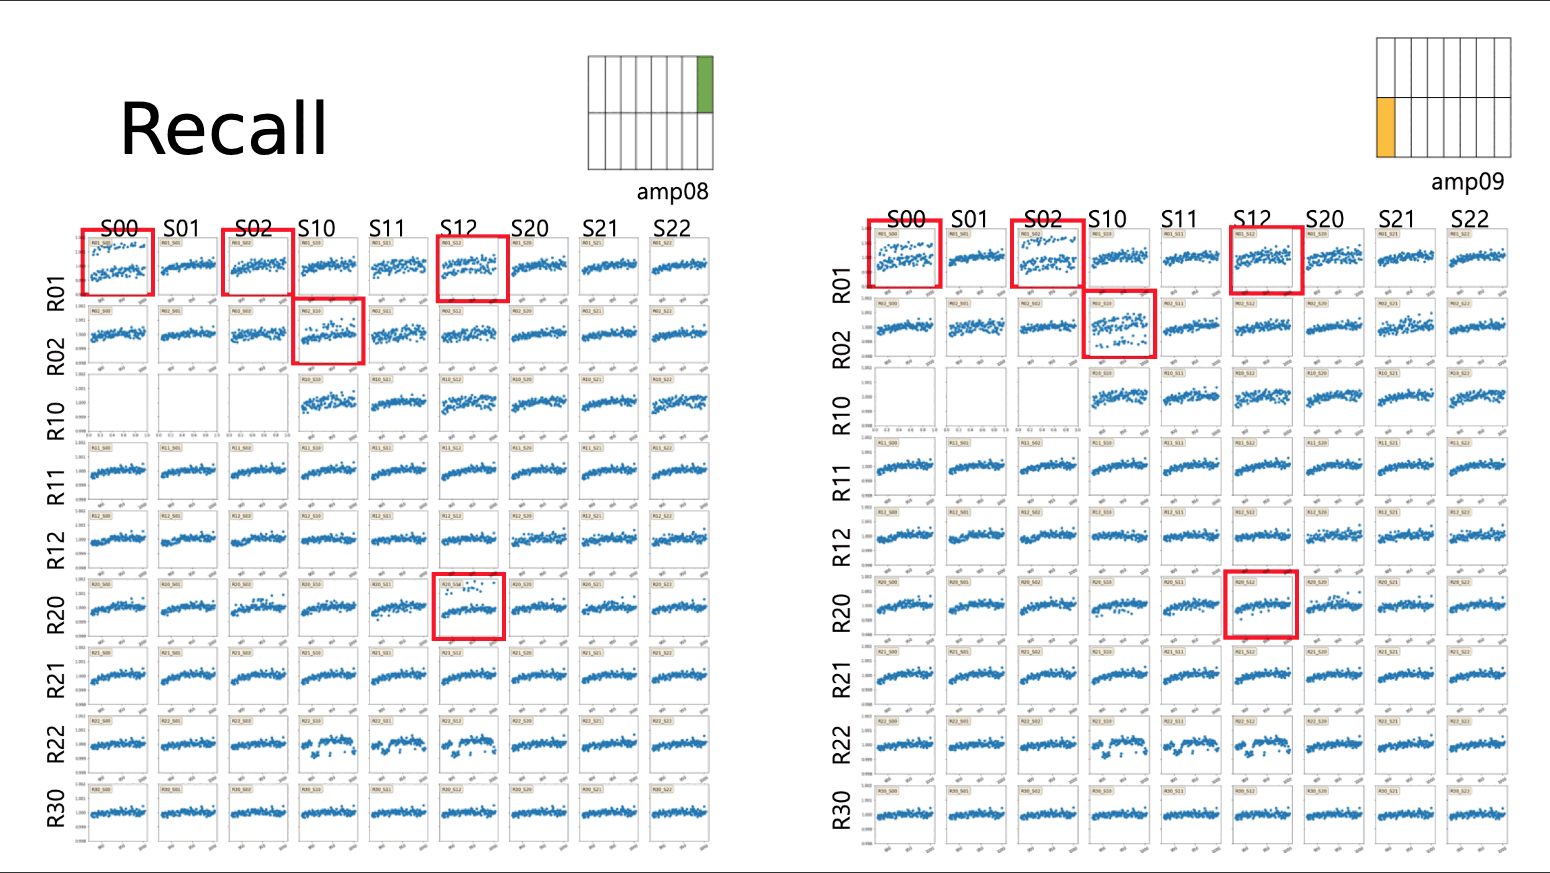
\includegraphics[width=0.9\textwidth]{sequencer/naturalfrequency/fig03_gainjump_recall_map.png}
\caption{Gain measurements per sensor across the focal plane for two amplifiers (amp08, left;
amp09, right). Red boxes mark sensors in which the gain moves between discrete states from one
acquisition to the next; the difference between states is at the sub-percent level.}
\label{fig:nf-gain-jump-recall}
\end{centering}
\end{figure}

The bias frames showed a related behaviour: they occupied distinct states in bias level, noise
and row profile, which meant that a super-bias built by averaging many frames could not be used
reliably. The effect is visible both as separate clusters in the plane of overscan noise versus
mean image level and as discrete bands in the overscan noise as a function of time
(Figure~\ref{fig:nf-bias-multimodality}), and it was reported independently in the analyses of
Shuang Liang and Thibault Guillemin.

\begin{figure}[htbp]
\begin{centering}
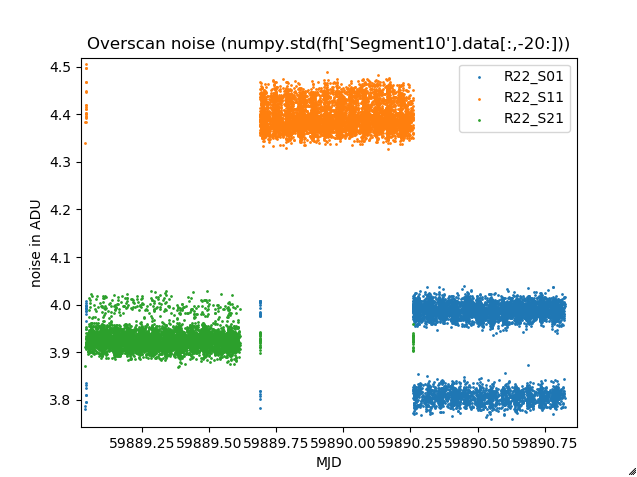
\includegraphics[width=0.48\linewidth]{sequencer/naturalfrequency/fig04a_shuang_overscan_noise_vs_mjd.png}
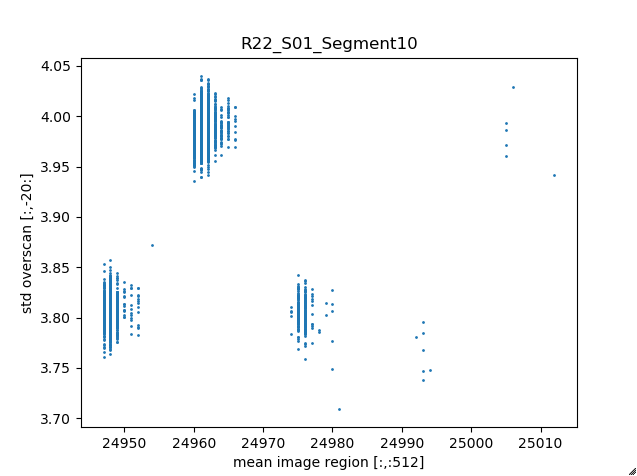
\includegraphics[width=0.48\linewidth]{sequencer/naturalfrequency/fig04b_shuang_std_vs_mean_r22s01.png}
\caption{Bias multimodality before the natural frequency firmware. Left: overscan noise as a
function of time for three sensors of raft R22, showing discrete bands rather than a continuous
distribution. Right: overscan noise versus mean image level for R22\_S01, segment 10, where the
same behaviour appears as separate clusters.}
\label{fig:nf-bias-multimodality}
\end{centering}
\end{figure}

%% NOTE: the two figures below are screenshots taken from a presentation and from a Slack thread
%% rather than plots regenerated for this note. They are kept here, commented out, in case the
%% original figures can be recovered from the authors; the text above and Figures
%% \ref{fig:nf-checkerboard-self} and \ref{fig:nf-covariance-grid} carry the same information.
%
% \begin{figure}[htbp]
% \begin{centering}
% 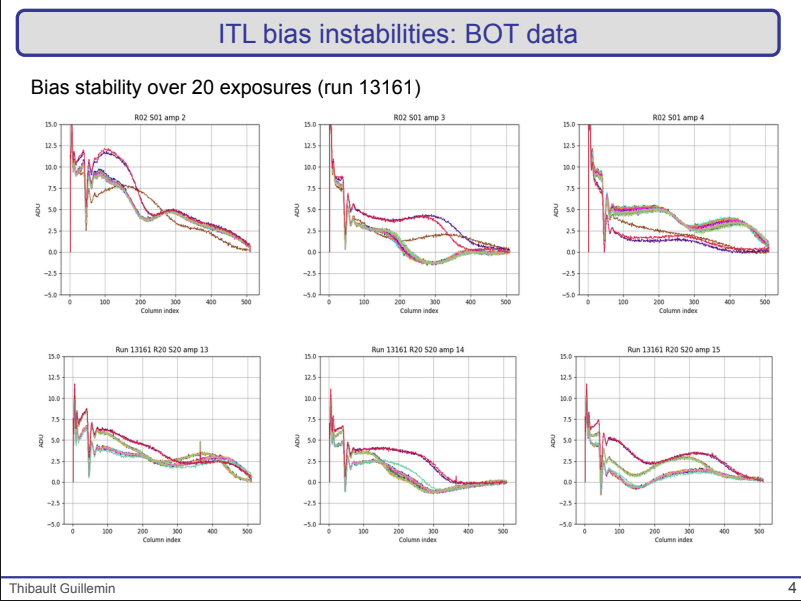
\includegraphics[width=0.8\textwidth]{sequencer/naturalfrequency/fig04c_thibault_itl_bias_instabilities.png}
% \caption{ITL bias instabilities in BOT data: bias row profiles over 20 exposures of run 13161
% for six amplifiers (T.~Guillemin).}
% \label{fig:nf-itl-bias-instabilities}
% \end{centering}
% \end{figure}
%
% \begin{figure}[htbp]
% \begin{centering}
% 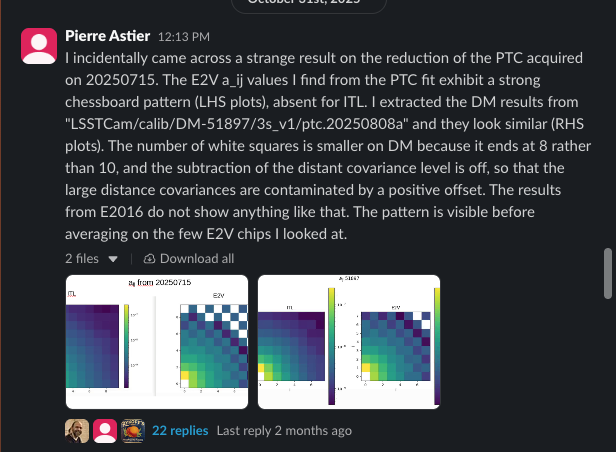
\includegraphics[width=0.8\textwidth]{sequencer/naturalfrequency/fig05_slack_checkerboard_aij_e2v_itl.png}
% \caption{Checkerboard pattern in the \(a_{ij}\) coefficients derived from the PTC acquired on
% 20250715, present for e2v and absent for ITL (P.~Astier).}
% \label{fig:nf-checkerboard-slack}
% \end{centering}
% \end{figure}

The third feature is the checkerboard, or chessboard, pattern that appears in the noise when
differences of pairs of PTC or overscan frames are correlated. In the notation used for the
covariance coefficients, \(n_{00}\) is the noise itself while \(n_{i0}\) traces CTI or a
gain variation, so a regular alternation of the covariance with pixel lag directly pollutes the
\(a_{ij}\) measurement. The pattern was strong for e2v sensors and essentially absent for ITL.

%%
%% Idea of the natural frequency
%%
A presentation by P.~Antilogus on 7 May 2024 proposed an explanation and gave the project its
name. There are two points in the readout chain at which an uncontrolled phase shift can be
introduced between the clocks of different REBs:

\begin{itemize}
    \item Each REB clock (6.4\,ns) is synchronized by the 3.125\,GHz common clock. An arbitrary
    phase shift, a multiple of a unit of 6.4\,ns/20, can be introduced at synchronization and
    persists until a link reset.
    \item A REB converts its 6.4\,ns clock to the 10\,ns clock used by the FPGA that runs the
    sequencer. A random phase shift of up to 10\,ns can be introduced at this conversion, and it
    can differ from one exposure to the next.
\end{itemize}

If the discrete states of the gain and of the bias arise from these phase shifts, then running
the REB at its natural frequency, that is, taking the sequencer timing directly from the 6.4\,ns
clock instead of the converted 10\,ns clock, should remove them.

%%
%% Idea of even-odd
%%
The checkerboard pattern admits a separate and complementary interpretation, proposed by the
French team: the regular pattern can be produced by a pair of clocks that carry a slight time
difference between them while their overall timing remains the same. If the ramp time takes an
odd number of clock cycles and the number of columns is odd, the alternation between the two
clocks maps onto the pixel grid and generates a checkerboard
(Figure~\ref{fig:nf-even-odd}). P.~Antilogus produced the \texttt{even2} sequencer file, in which
all the relevant time periods take an even number of cycles. This sequencer, carrying both the
even--odd change and the natural frequency timing, was subsequently adopted as the production
sequencer under the name \texttt{3s-v2} (calibration tag \texttt{3s\_v2}), superseding
\texttt{3s-v1}.

\begin{figure}[htbp]
\begin{centering}
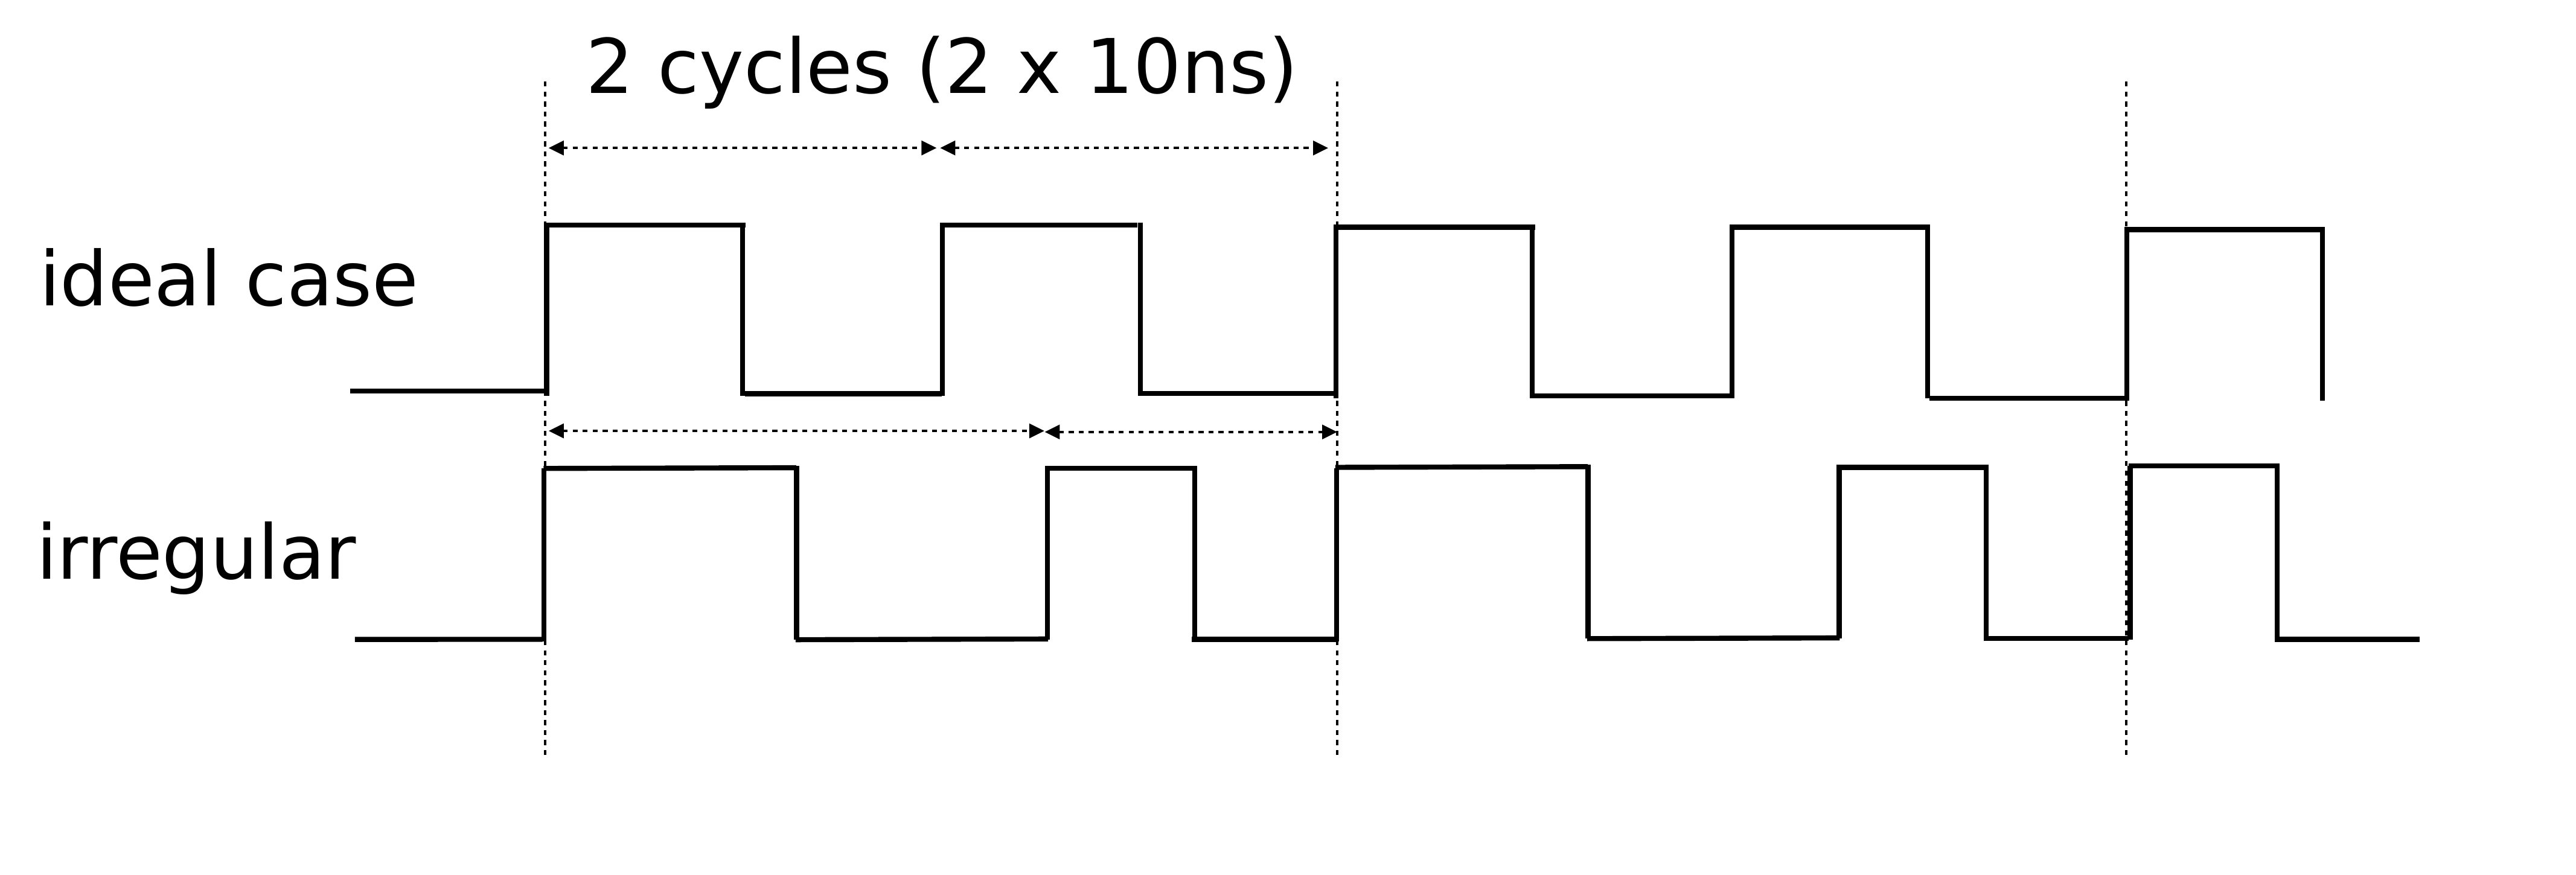
\includegraphics[width=0.85\textwidth]{sequencer/naturalfrequency/fig07_even_odd_diagram.png}
\caption{Schematic of the even--odd effect. In the ideal case (top) each period of the readout
covers two full clock cycles (2\(\,\times\,\)10\,ns). When the number of cycles is odd (bottom),
successive periods start on alternating clock phases, so consecutive columns are read with a
slightly different timing.}
\label{fig:nf-even-odd}
\end{centering}
\end{figure}

\clearpage

%%
%% Firmware and validation
%%
The natural frequency operation is provided by Science REB firmware 0x313B5019, released in
December 2025 and listed in Table~\ref{tab:science_reb_fw_en}. That release completes the code
refactor which allows the system clock to be chosen on a per-target basis using a common set of
functional blocks, so that the same VHDL code serves both the 6.4\,ns and the 10\,ns cases with
only a parameter change. The same libraries can now be used in the WREB and GREB firmware, and
the remaining work is to apply them to the devices unique to those boards.

Validation was organized by board type. For the Science REBs, the new firmware was tested on TS8
for ITL and at UC Davis for e2v before installation on the camera, with multimodality (100 biases)
and small PTC acquisitions; the run records are collected in the RTM-004 optimization runs page.
For the WREB, a 100-bias acquisition with LATISS revealed an oddity that paused the deployment
(see the LATISS testing discussed below). For the GREB, firmware development is still underway.
The configuration adopted for the campaigns reported here is therefore the natural frequency
firmware with the \texttt{3s-v2} sequencer for the science rafts, and the original firmware for
the WREB and GREB. J.~Chiang ran the \texttt{cp}/\texttt{eo} pipelines promptly on each
acquisition, and the individual analyses below were carried out on those outputs.

%%
%% Testing campaigns: both the bias/flat campaign and the PTC/linearizer acquisitions
%%
\paragraph{Testing campaigns.}
The bias and flat campaign comprised the following acquisitions:

\begin{itemize}
    \item Biases, 9 December 2025, sequence numbers 13--112.
    \item Flat stability, 14 December 2025:
    \begin{itemize}
        \item Gain stability (BLOCK-T661): 11--110, 100 flats targeting 12\,k\(e^-\); 111--210,
        100 flats targeting 50\,k\(e^-\); 514--613, 100 flats targeting 12\,k\(e^-\); 614--713,
        100 flats targeting 50\,k\(e^-\) (after sun down).
        \item Biases (BLOCK-T659), with an RCE reset between runs: 211--310, 313--412 and
        413--512, 100 biases each.
    \end{itemize}
    \item PTC, white light flats and darks on 27 December 2025 (taken with the mirror cover
    partially closed), 28 December 2025 (second attempt) and 3 January 2026.
    \item Science images, taken as a bonus on 3 January 2026.
\end{itemize}

A second, independent look at the same firmware came from the PTC and linearizer products, in an
analysis by E.~Rykoff reported in January 2026. Those data are the acquisitions of 29 December
2025, a full night with 524 flat pairs, processed into the collection
\texttt{LSSTCam/calib/DM-53722} under the tag \texttt{3s\_v2}. The pairs were shuffled in flux
order and no photodiode or electrometer reading was available, so that analysis is purely internal
to the CCDs; the signal range runs from roughly 50--100\,adu up through the PTC turnoff, except on
the corner detectors. The comparison set is the equivalent acquisition of 15 July 2025
(BLOCK-T557) with the same signal range and configuration, processed in
\texttt{LSSTCam/calib/DM-53620} under the tag \texttt{3s\_v1\_dp2\_v2}. Detector 122 is excluded
from both.

The linearizer fitter used for those products is an implementation of P.~Astier's linearizer fit
with modifications: it includes a global offset term and a linear temporal term, and it does not
use modified weights or the REB temperature (\texttt{TEMPAVG}). The fit is split into a
``relative'' and an ``absolute'' linearization. The least-squares minimizer was found to get
stuck, and applying the temporal fit together with the relative slopes and then re-fitting brought
it to a much better state; every one of the 3,024 amplifiers was inspected individually.

\clearpage

%%
%% Results: noise and gain consistency, from both directions
%%
\paragraph{Noise and gain consistency between configurations.}
The readout noise measured with the 6.4\,ns sequencer (\texttt{3s\_cp\_v1\_even2\_64}) and with
the 10\,ns sequencer (\texttt{3s\_cp\_v1}) agrees closely, with mean ratios of 1.003 for e2v and
0.991 for ITL (Figure~\ref{fig:nf-noise-consistency}). A small rounding in the sequencer timing
makes the gains inconsistent between vendors at the 1\% level. The outliers are half-dead or
high-noise sensors (R10\_S01, R43\_S20, R41\_S21). No geometrically systematic correlation across
the focal plane was observed, which addresses the concern that the WREB might inject noise into
neighbouring rafts.

\begin{figure}[htbp]
\begin{centering}
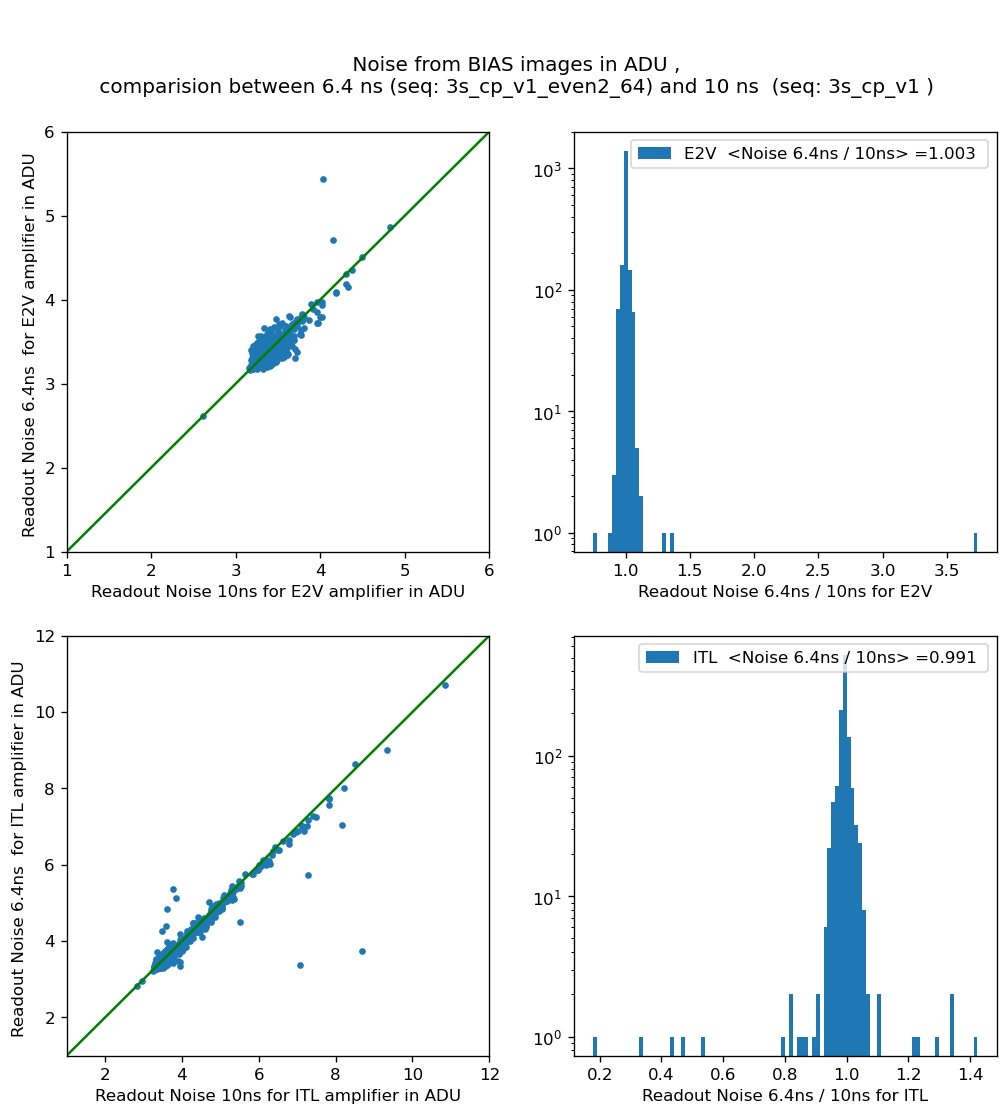
\includegraphics[width=0.75\textwidth]{sequencer/naturalfrequency/fig11_readout_noise_6p4ns_vs_10ns.png}
\caption{Readout noise from bias images, comparing the 6.4\,ns sequencer
(\texttt{3s\_cp\_v1\_even2\_64}) with the 10\,ns sequencer (\texttt{3s\_cp\_v1}), for e2v (top)
and ITL (bottom). Left: amplifier by amplifier. Right: distribution of the ratio between the two
(P.~Antilogus).}
\label{fig:nf-noise-consistency}
\end{centering}
\end{figure}

The PTC products give the same result from the flats, amplifier by amplifier across the whole
focal plane (Figure~\ref{fig:nf-ptc-gain-noise}). The gains move slightly and in opposite
directions for the two vendors, e2v down a little and ITL up a little, which is the vendor-
dependent rounding above seen in the gain itself rather than in the noise. The read noise
generally decreases for all amplifiers, and for a subset of e2v amplifiers it decreases
substantially --- presumably the channels that were carrying the excess variance associated with
the checkerboard discussed below.

\begin{figure}[htbp]
\begin{centering}
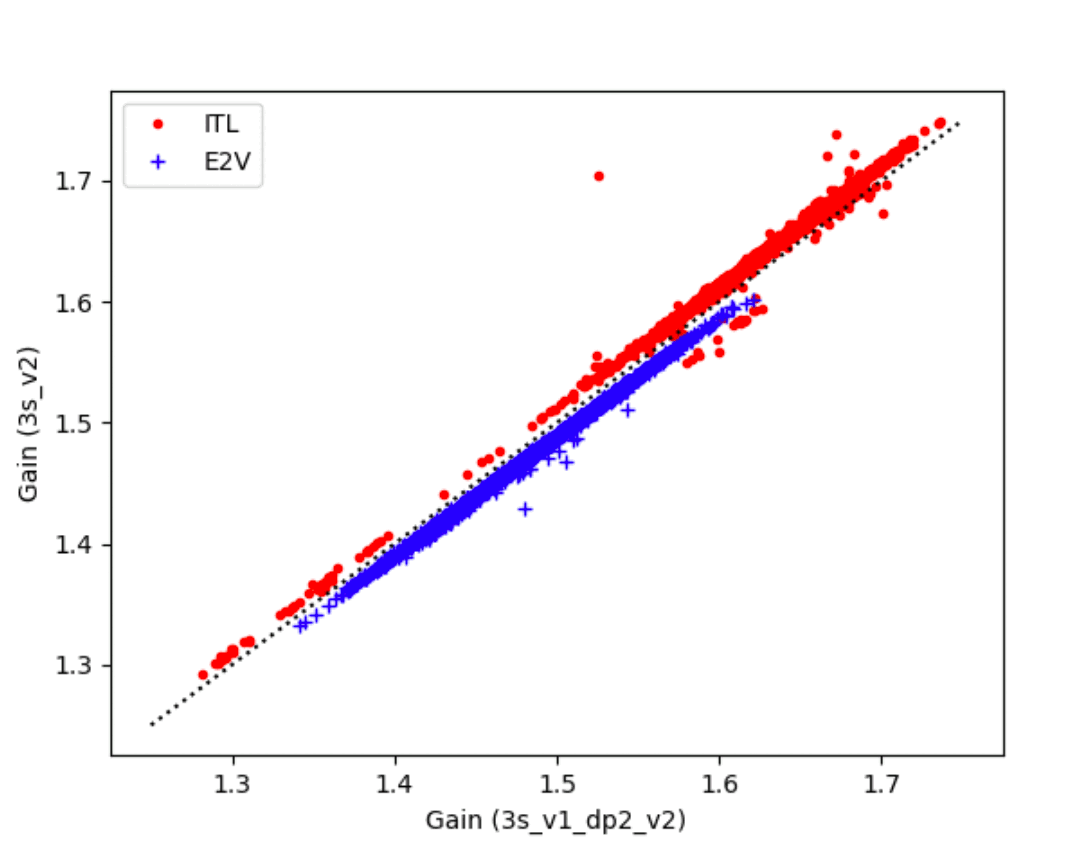
\includegraphics[width=0.48\linewidth]{sequencer/naturalfrequency/fig27a_gain_comparison.png}
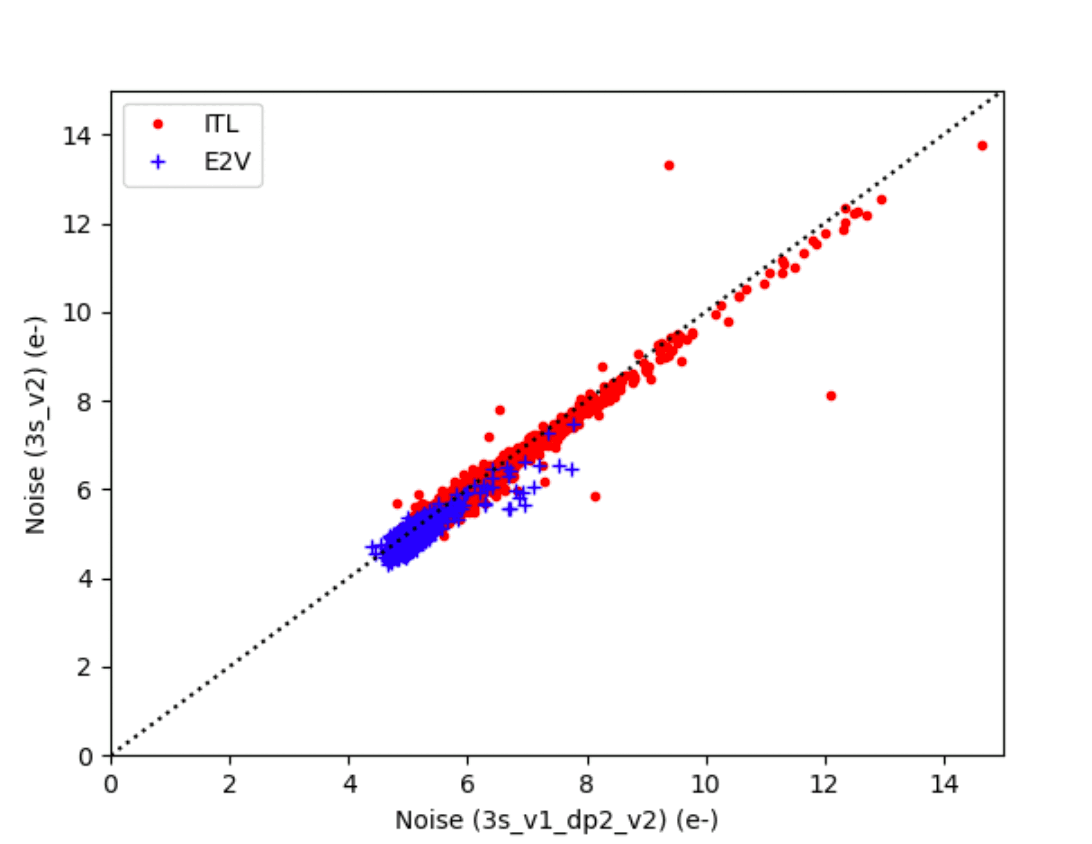
\includegraphics[width=0.48\linewidth]{sequencer/naturalfrequency/fig27b_noise_comparison.png}
\caption{Per-amplifier comparison between \texttt{3s\_v1\_dp2\_v2} and \texttt{3s\_v2} from the
PTC. Left: gain. Right: read noise in electrons. The dotted line is equality (E.~Rykoff).}
\label{fig:nf-ptc-gain-noise}
\end{centering}
\end{figure}

\clearpage

%%
%% Results: bias multimodality
%%
\paragraph{Bias level versus noise.}
Plotting the overscan noise against the overscan mean for one amplifier per sensor over the whole
focal plane (Figure~\ref{fig:nf-bias-vs-noise}) no longer shows multiple distinct populations. The
residual systematic drift within each sensor is consistent with gain and temperature changes over
the duration of the acquisition rather than with discrete state changes.

\begin{figure}[htbp]
\begin{centering}
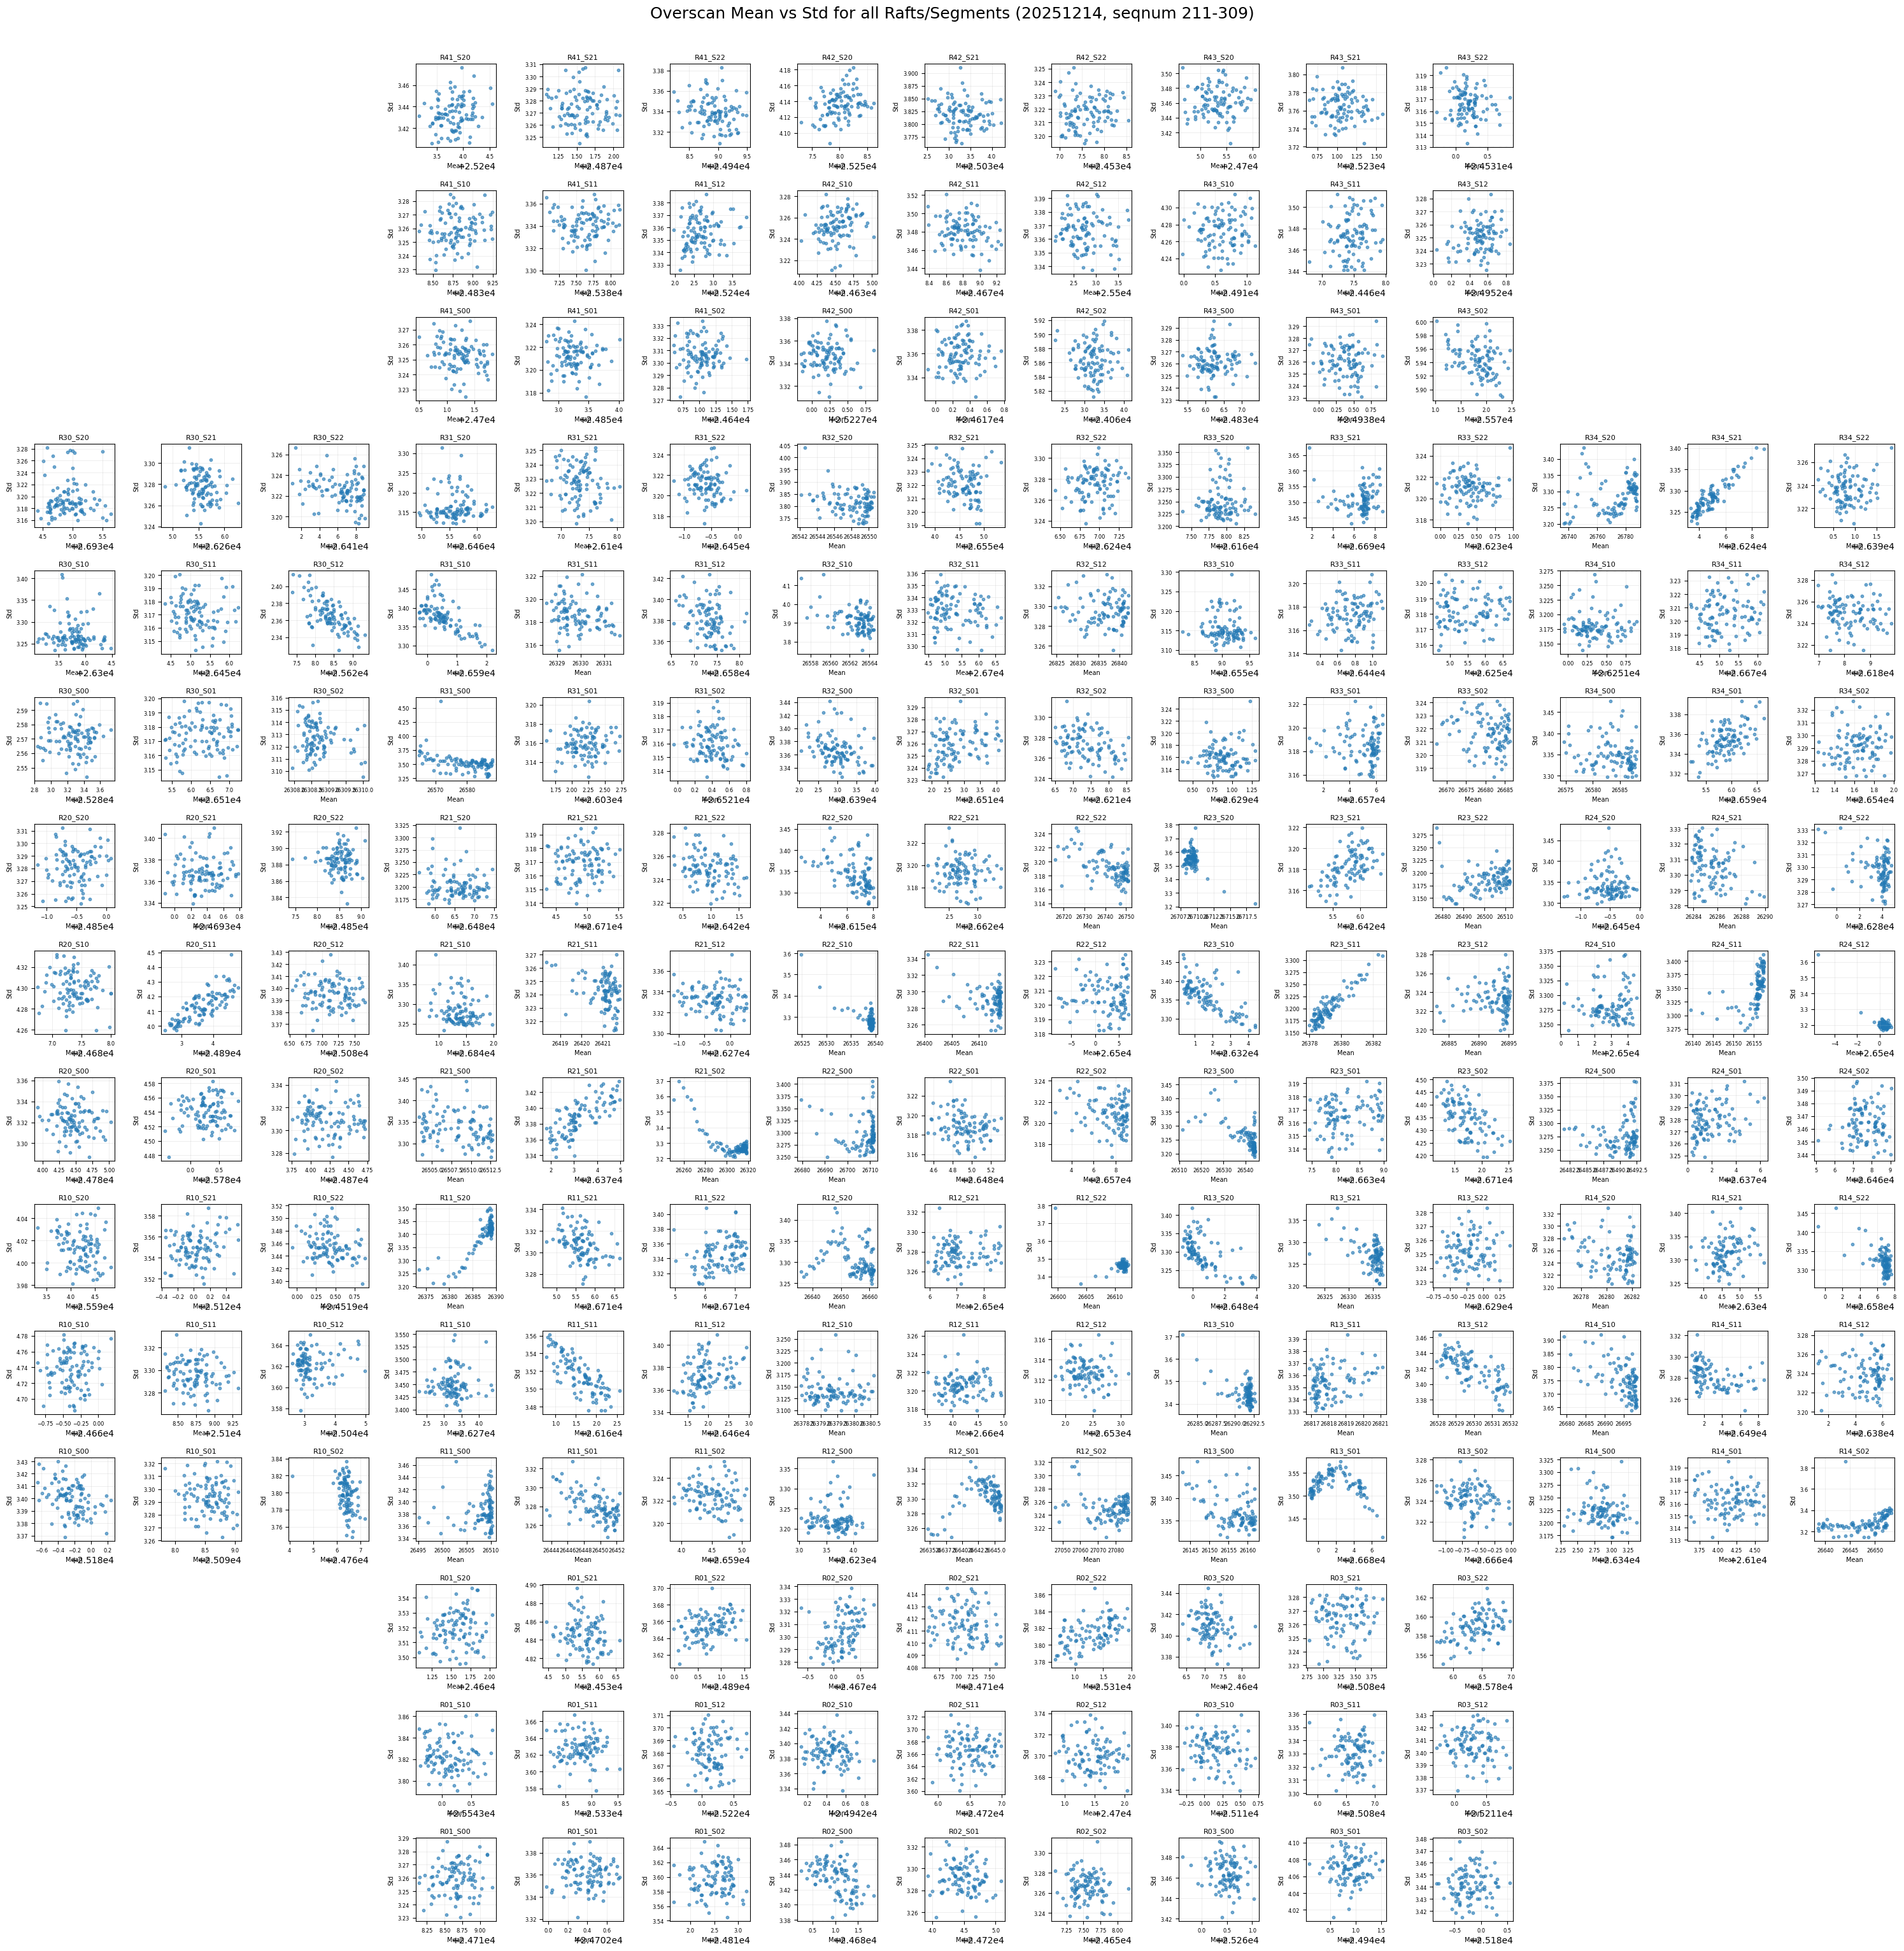
\includegraphics[width=0.95\textwidth]{sequencer/naturalfrequency/fig12_overscan_mean_vs_std_focalplane.png}
\caption{Overscan mean versus overscan standard deviation for all rafts and sensors
(20251214, sequence numbers 211--309), one amplifier per sensor. The distinct populations seen
before the firmware change (Figure~\ref{fig:nf-bias-multimodality}) are absent.}
\label{fig:nf-bias-vs-noise}
\end{centering}
\end{figure}

\paragraph{Bias row profiles.}
The row profiles measured before and after the change are compared in
Figure~\ref{fig:nf-row-profiles}. With the original firmware the profile of a given amplifier
differed between exposures; with the natural frequency firmware the profiles from repeated
exposures fall on top of each other.

\begin{figure}[htbp]
\begin{centering}
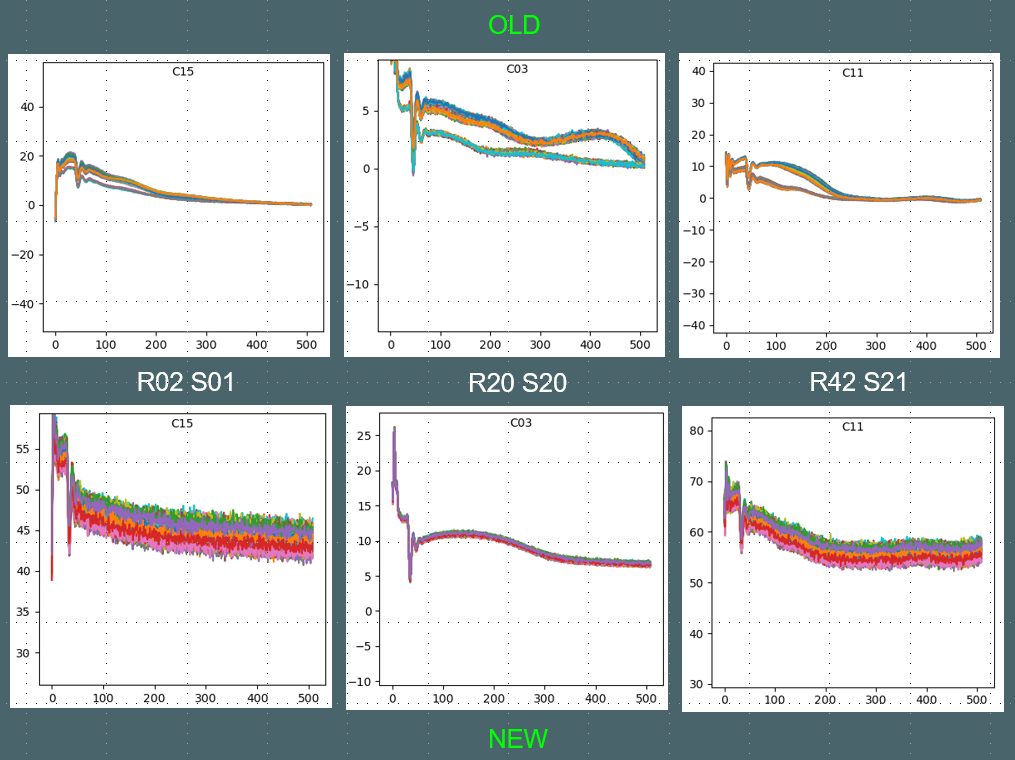
\includegraphics[width=0.85\textwidth]{sequencer/naturalfrequency/fig13_row_profiles_old_vs_new.png}
\caption{Bias row profiles for three amplifiers (R02\_S01 C15, R20\_S20 C03, R42\_S21 C11) with
the original firmware (top) and with the natural frequency firmware (bottom, run E1110, 9
December 2025). The profiles become consistent from exposure to exposure (T.~Guillemin).}
\label{fig:nf-row-profiles}
\end{centering}
\end{figure}

\paragraph{Consistency across resets.}
Since the phase shift introduced at REB synchronization persists until a link reset, the
acquisitions of 14 December 2025 were split into three runs separated by an RCE reset. The mean
parallel overscan profiles of the three runs agree amplifier by amplifier
(Figure~\ref{fig:nf-reset-consistency}); no change was observed between before and after a reset.
Together with the noise agreement above, this points at the 6.4\,ns to 10\,ns conversion rather
than at the REB synchronization as the origin of the multimodality.

\begin{figure}[htbp]
\begin{centering}
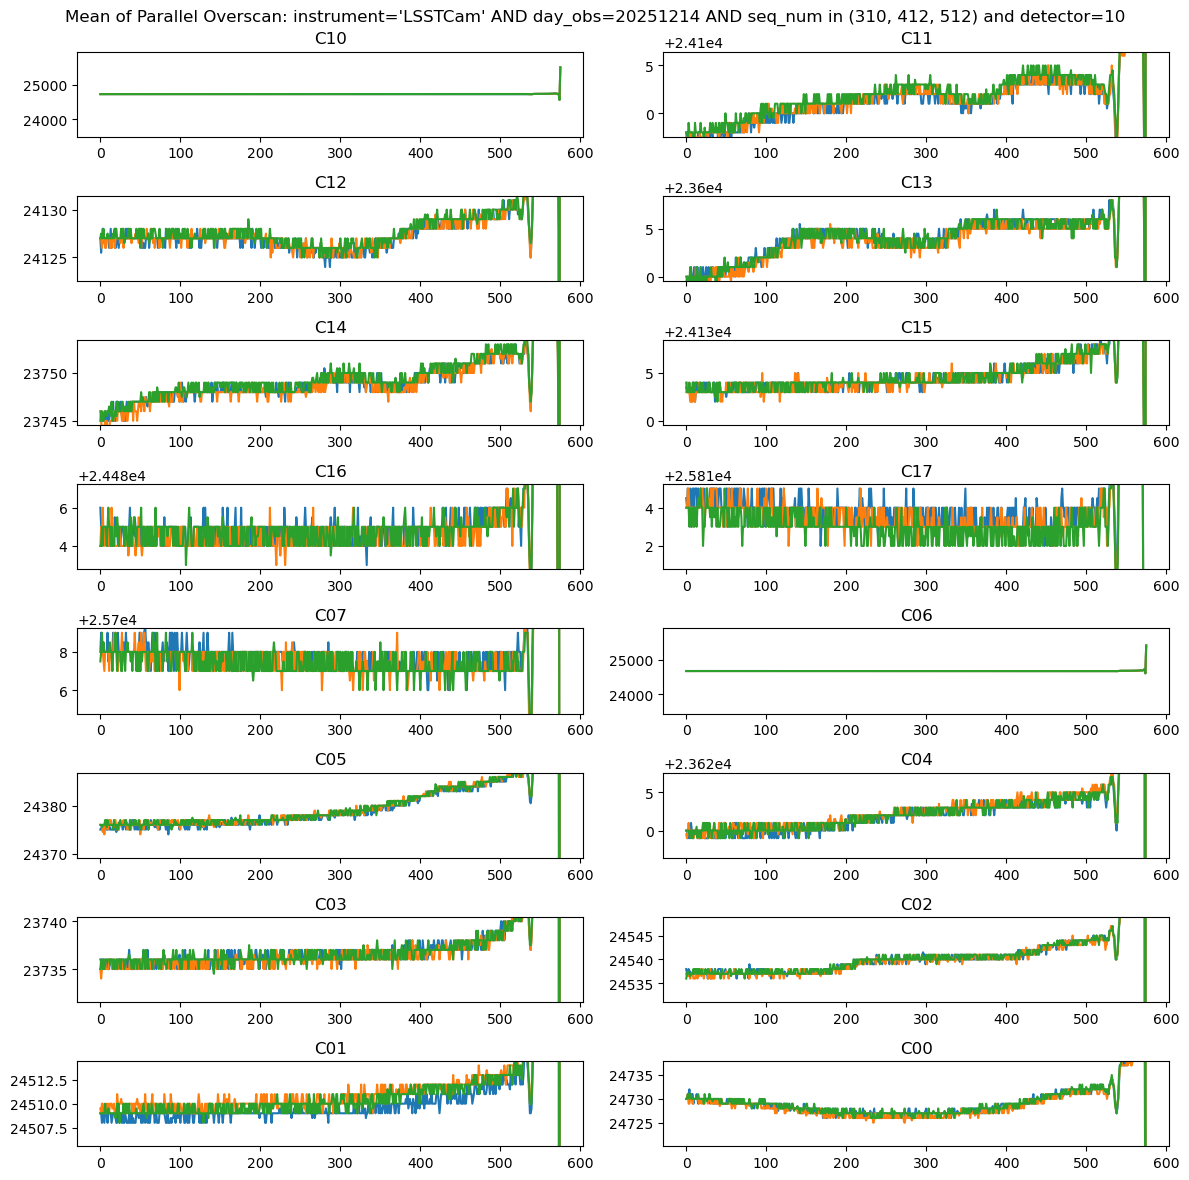
\includegraphics[width=0.85\textwidth]{sequencer/naturalfrequency/fig14_parallel_overscan_reset_consistency.png}
\caption{Mean of the parallel overscan for each amplifier of detector 10, for the three runs of
20251214 separated by an RCE reset (sequence numbers 310, 412 and 512). The three curves overlap
in every channel.}
\label{fig:nf-reset-consistency}
\end{centering}
\end{figure}

\clearpage

%%
%% Results: gain stability
%%
\paragraph{Gain stability.}
The relative gain change of every amplifier, measured against the focal-plane median, is shown in
Figure~\ref{fig:nf-gain-jumps} without and with the natural frequency firmware. Without it the
median gain drifts by more than \(2\times10^{-3}\) over the run; with it the drift is removed and
the residual per-amplifier scatter is at the level of the measurement noise. The amplifiers that
remain noisy in the right-hand panel are noisy intrinsically.

\begin{figure}[htbp]
\begin{centering}
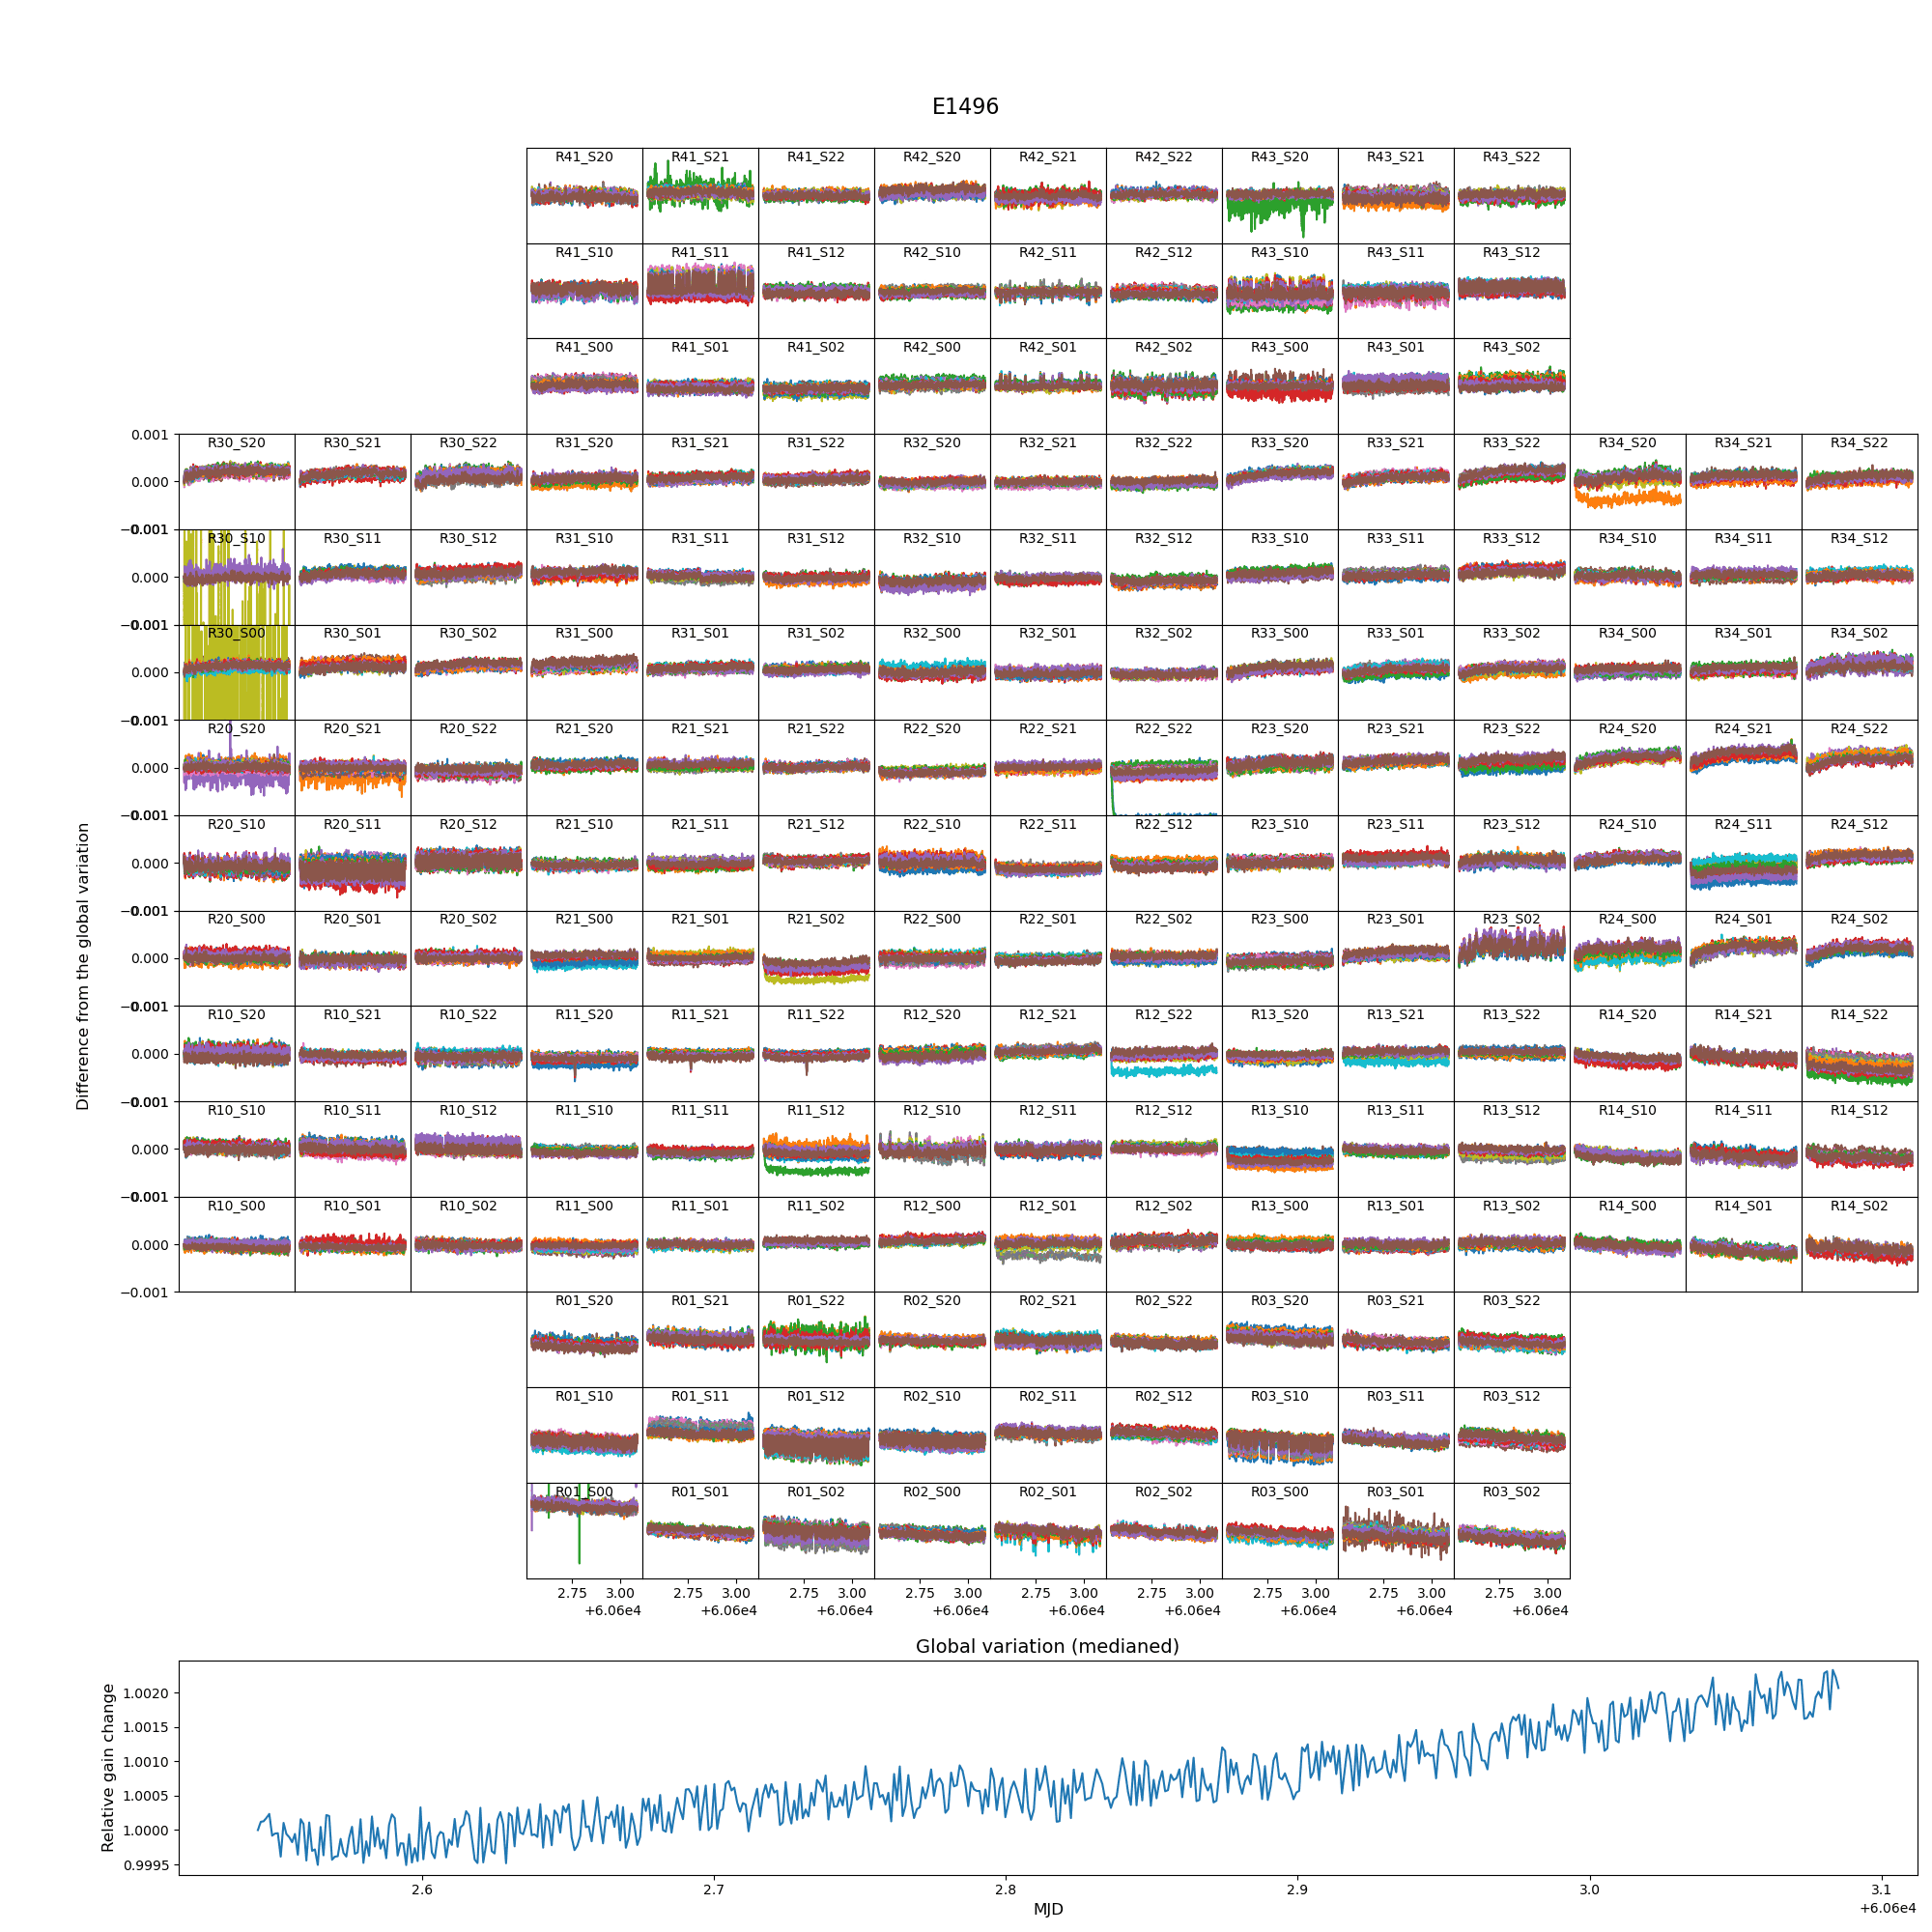
\includegraphics[width=0.48\linewidth]{sequencer/naturalfrequency/fig15a_gain_jumps_wo_naturalfreq_e1496.png}
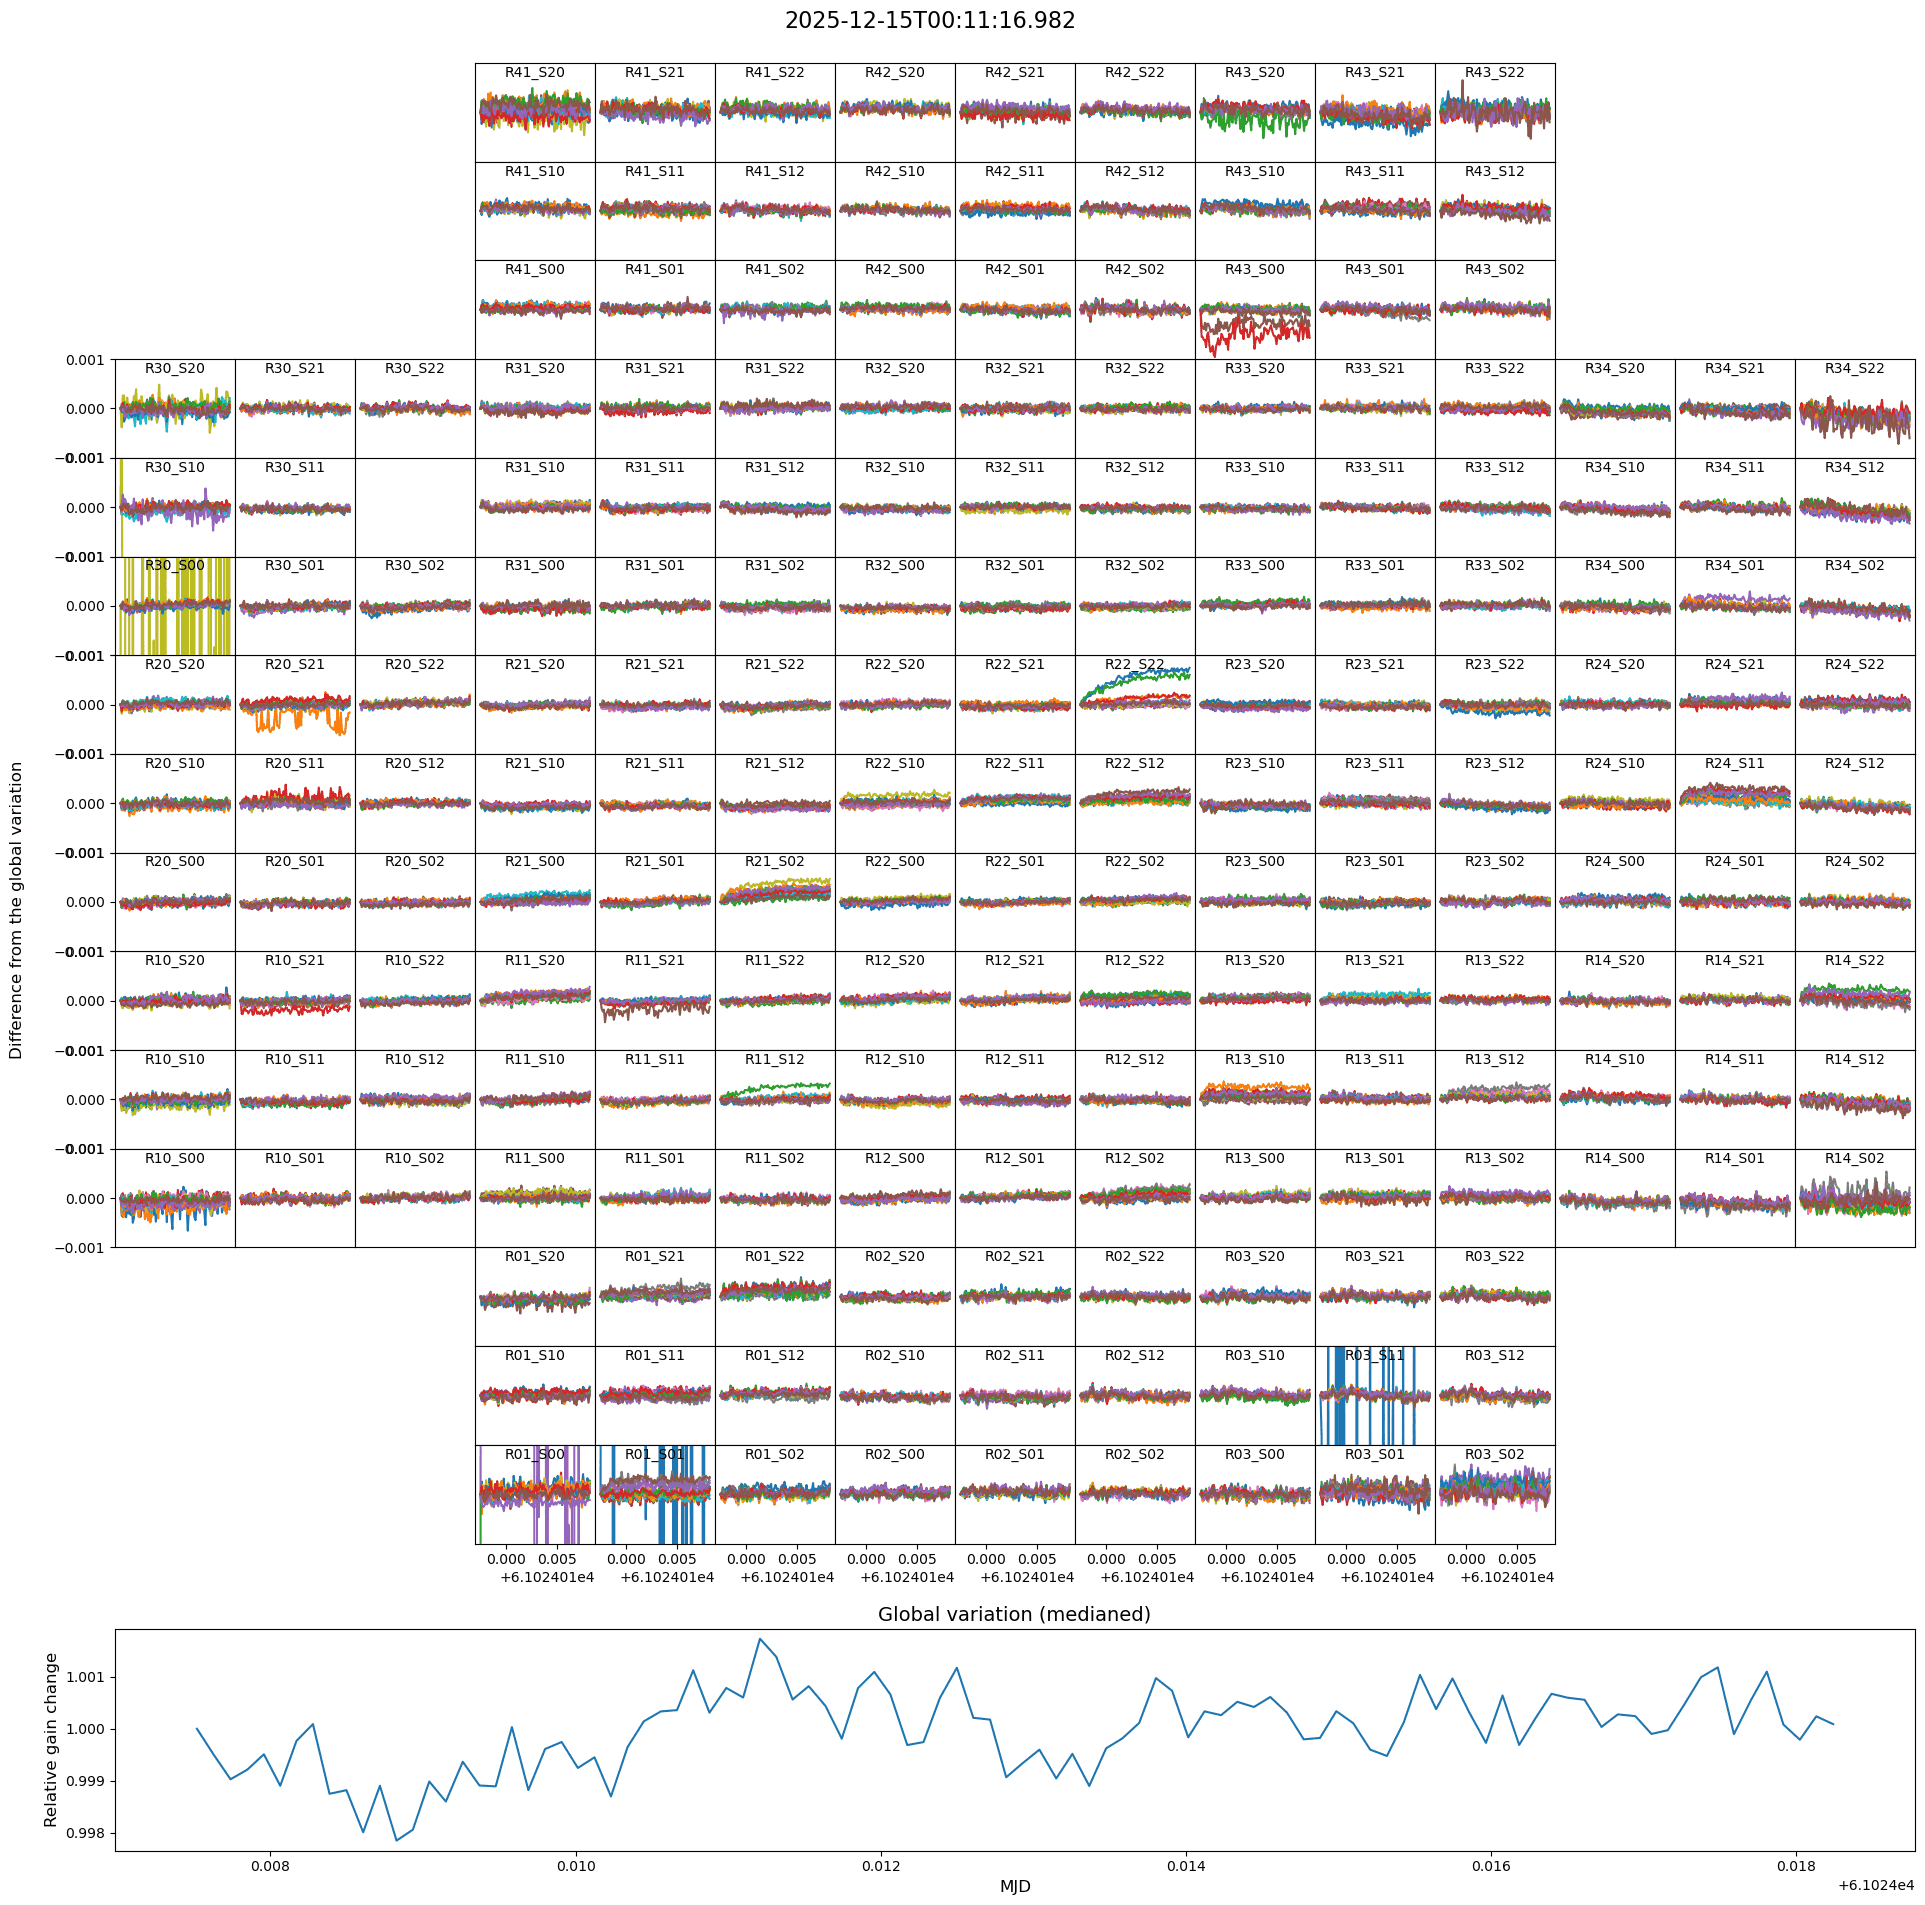
\includegraphics[width=0.48\linewidth]{sequencer/naturalfrequency/fig15b_gain_jumps_w_naturalfreq.png}
\caption{Difference of the per-amplifier relative gain from the focal-plane median, and the
median itself (bottom panel of each plot). Left: without the natural frequency firmware (run
E1496). Right: with the natural frequency firmware (2025-12-15).}
\label{fig:nf-gain-jumps}
\end{centering}
\end{figure}

The same measurement performed on the high-flux flats
(Figure~\ref{fig:nf-gain-jumps-highflux}) is to be compared with the specification of 0.1\% RMS
over 1\,h and 1\% RMS over 12\,h. The majority of the amplifiers are better than
\(\mathcal{O}(10^{-4})\). Three classes of outlier remain: non-stable illumination at the edge of
the focal plane, sensor-intrinsic behaviour, and a gain--temperature correlation that is not yet
understood. The linearity analysis below finds residual patterns of exactly these two kinds ---
smooth variation over the night on the vignetted edge detectors, and a time and temperature
correlation on isolated amplifiers --- which suggests the two campaigns are seeing the same
residual effects through different measurements.

\begin{figure}[htbp]
\begin{centering}
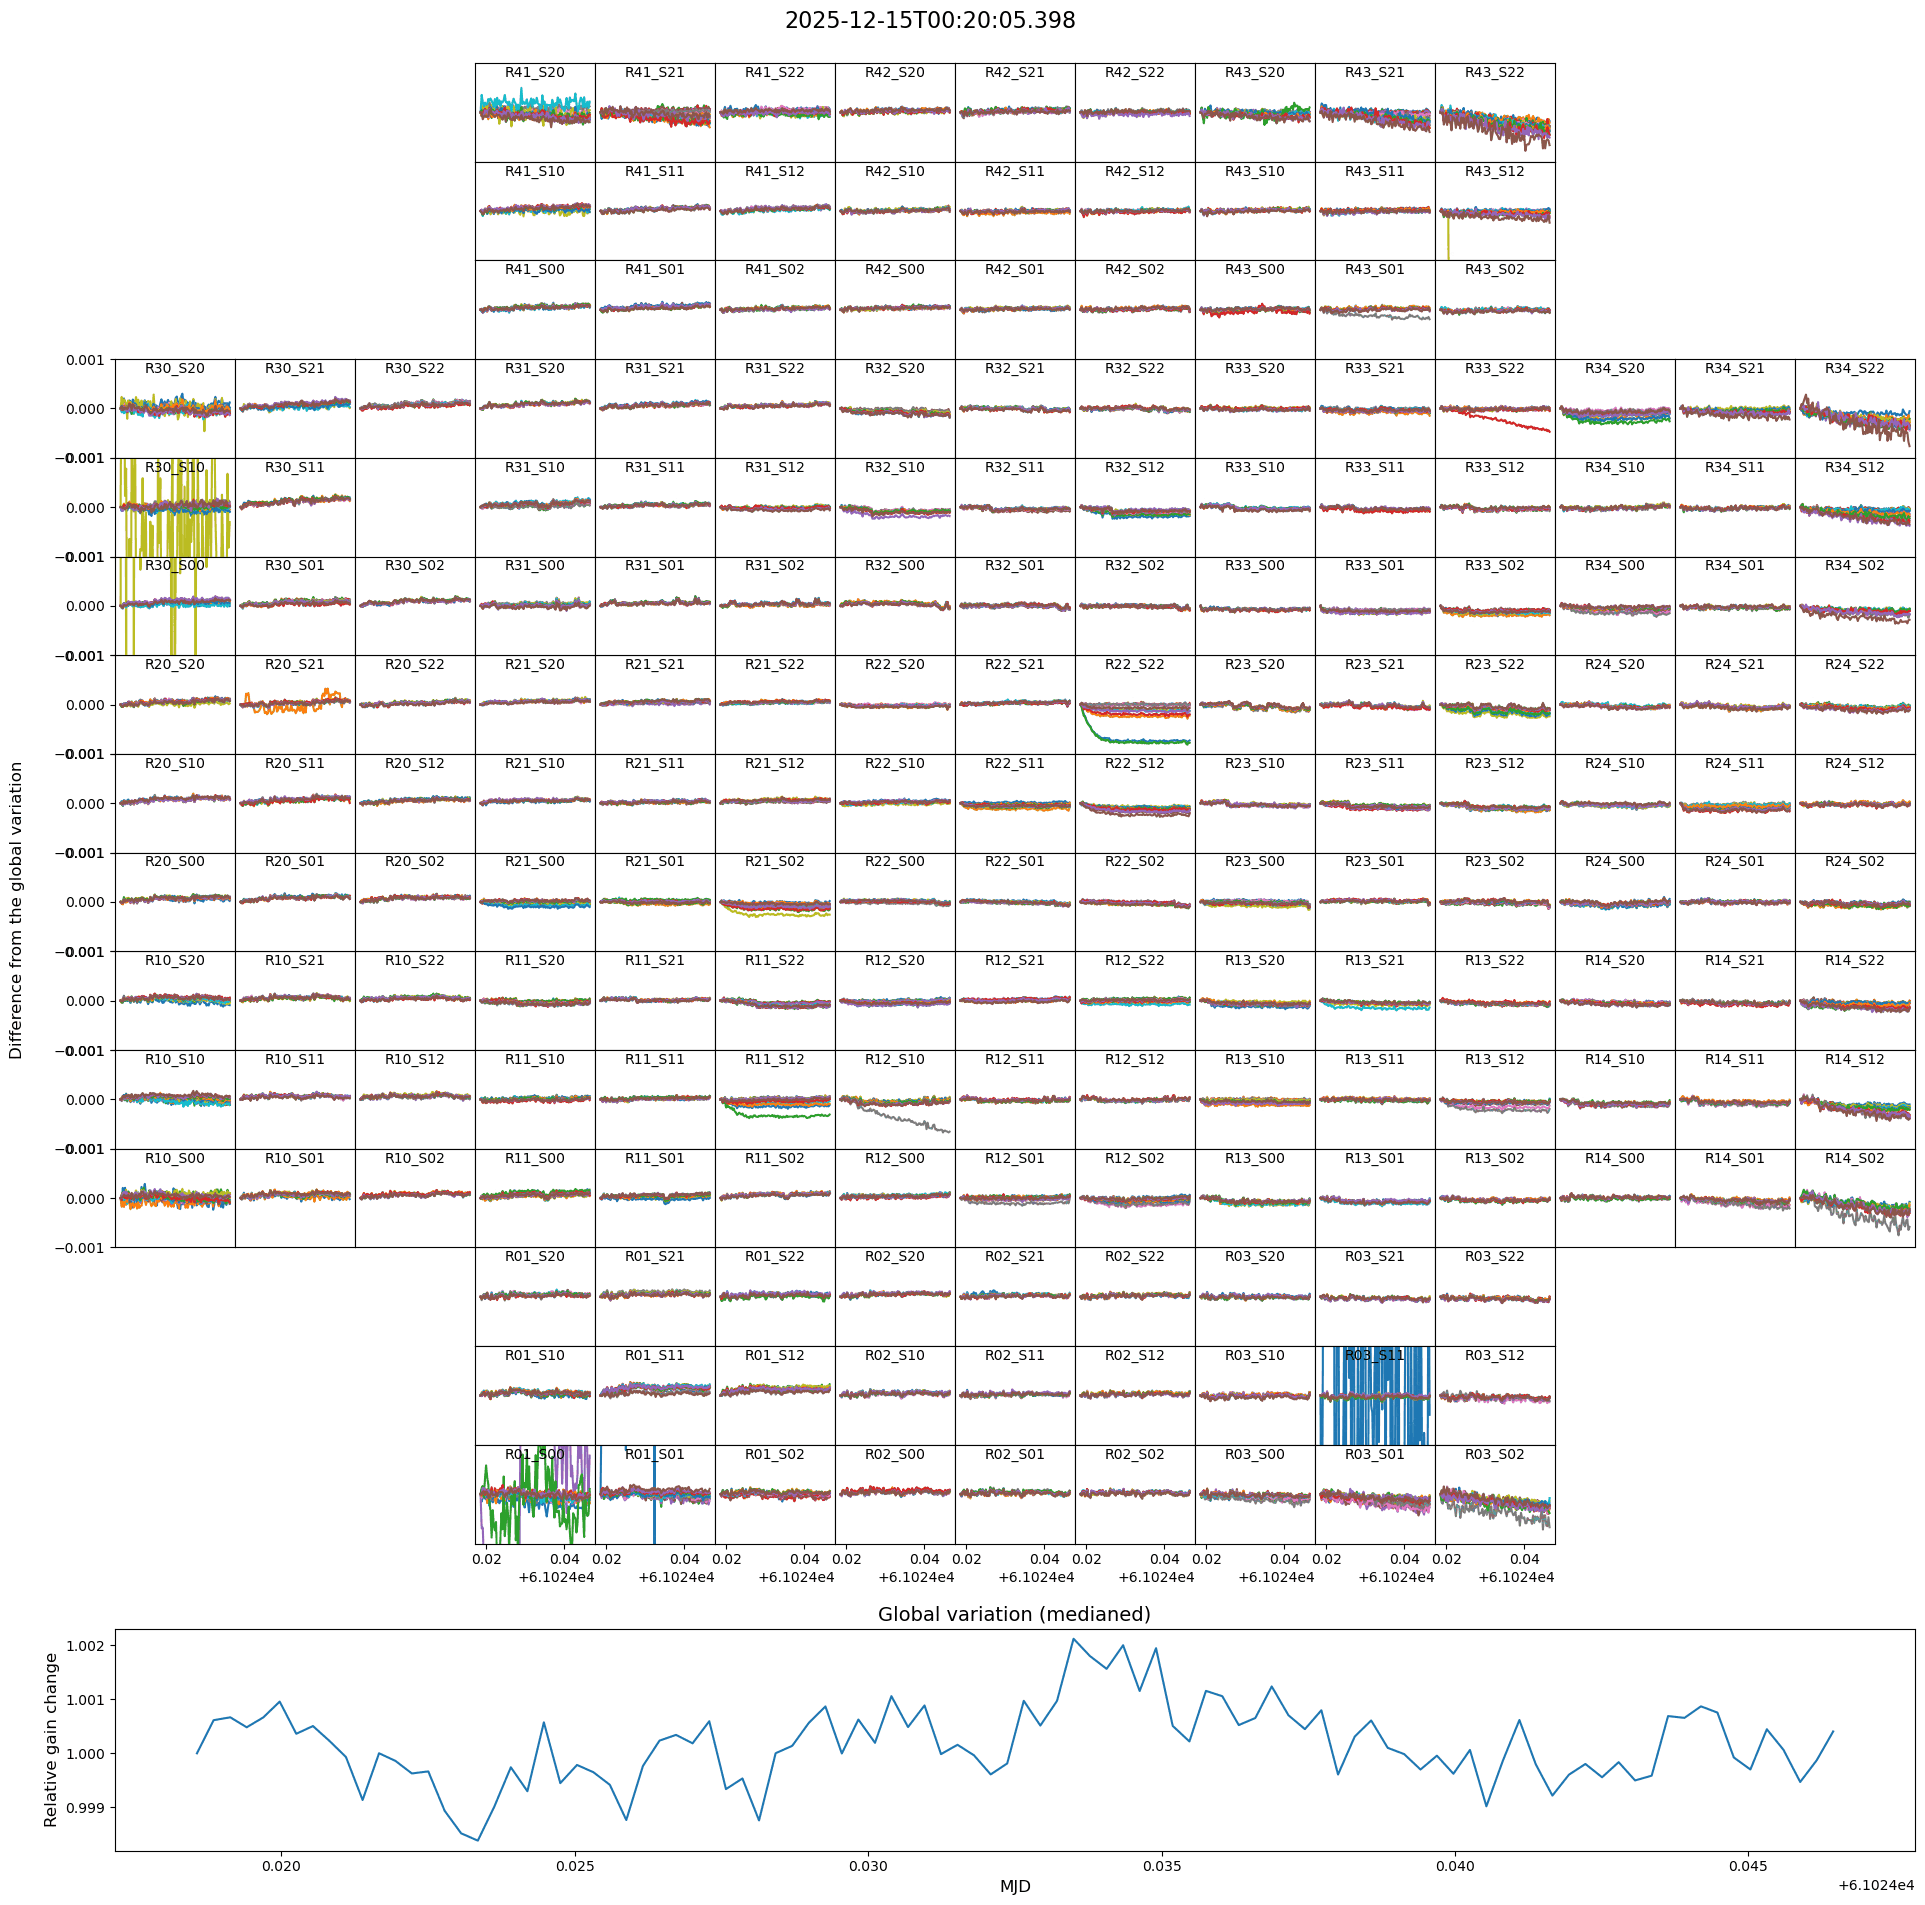
\includegraphics[width=0.95\textwidth]{sequencer/naturalfrequency/fig16_gain_jumps_highflux.png}
\caption{Relative gain change per amplifier for the high-flux flats acquired with the natural
frequency firmware (2025-12-15), in the same format as Figure~\ref{fig:nf-gain-jumps}.}
\label{fig:nf-gain-jumps-highflux}
\end{centering}
\end{figure}

\clearpage

%%
%% Results: checkerboard, from the overscan and from the PTC
%%
\paragraph{Checkerboard in the overscan.}
The two-dimensional lagged correlation of the serial overscan, averaged over all amplifiers of
R23\_S02, is shown in Figure~\ref{fig:nf-checkerboard-self} for the original and for the natural
frequency configuration. The checkerboard pattern is gone in the latter.

\begin{figure}[htbp]
\begin{centering}
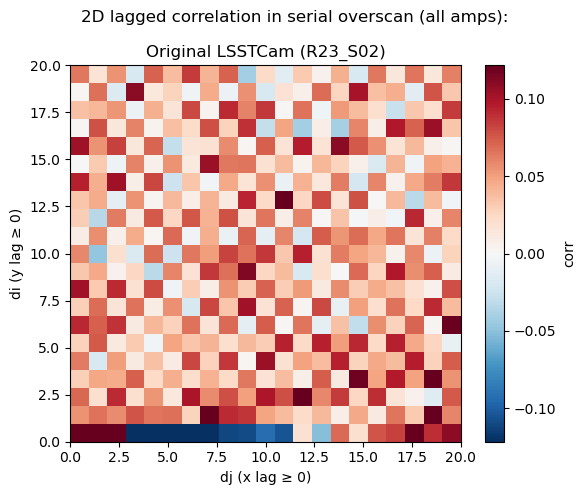
\includegraphics[width=0.48\linewidth]{sequencer/naturalfrequency/fig17a_checkerboard_original.png}
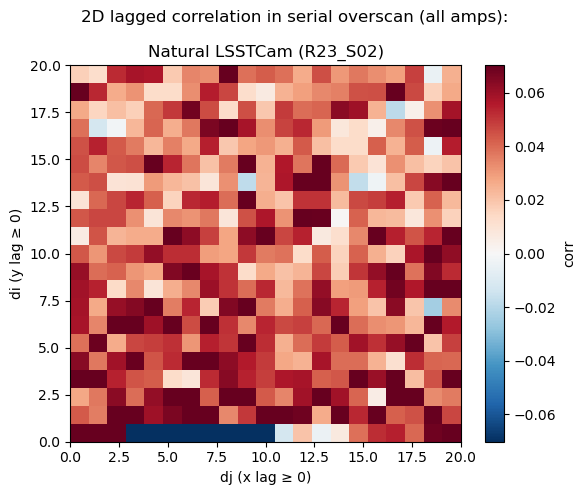
\includegraphics[width=0.48\linewidth]{sequencer/naturalfrequency/fig17b_checkerboard_natural.png}
\caption{Two-dimensional lagged correlation in the serial overscan, all amplifiers of R23\_S02.
Left: original configuration (20251216, sequence number 366). Right: natural frequency
configuration (20251214, sequence number 211).}
\label{fig:nf-checkerboard-self}
\end{centering}
\end{figure}

Figure~\ref{fig:nf-covariance-grid} shows the covariances \(\langle \mathrm{cov}_{ij} \rangle\)
for all channel pairs of R23\_S02, excluding the self-correlations, before and after the change.
The average over pairs, shown as an inset, carries a clear checkerboard in the original data and
is flat with the natural frequency firmware. P.~Astier interpreted the decaying signal at
\(\Delta y = 0\) as a gain variation, which the natural frequency partially cures: the spread of
the relative gain of R23\_S02 narrows from roughly \(\pm10^{-3}\) to a considerably smaller range
(Figure~\ref{fig:nf-relative-gain-insets}).

\begin{figure}[htbp]
\begin{centering}
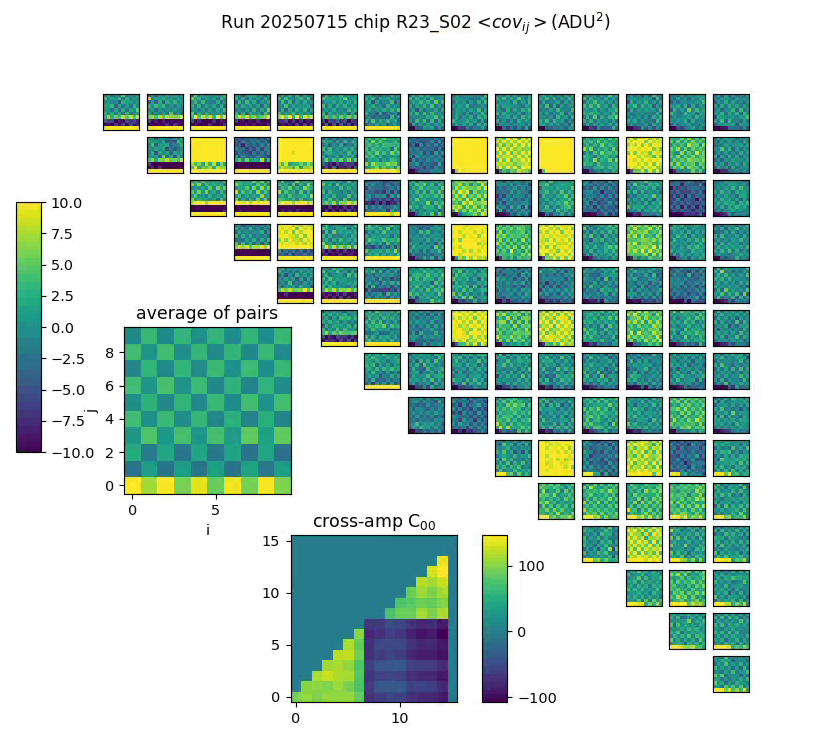
\includegraphics[width=0.48\linewidth]{sequencer/naturalfrequency/fig18a_covariance_grid_original.png}
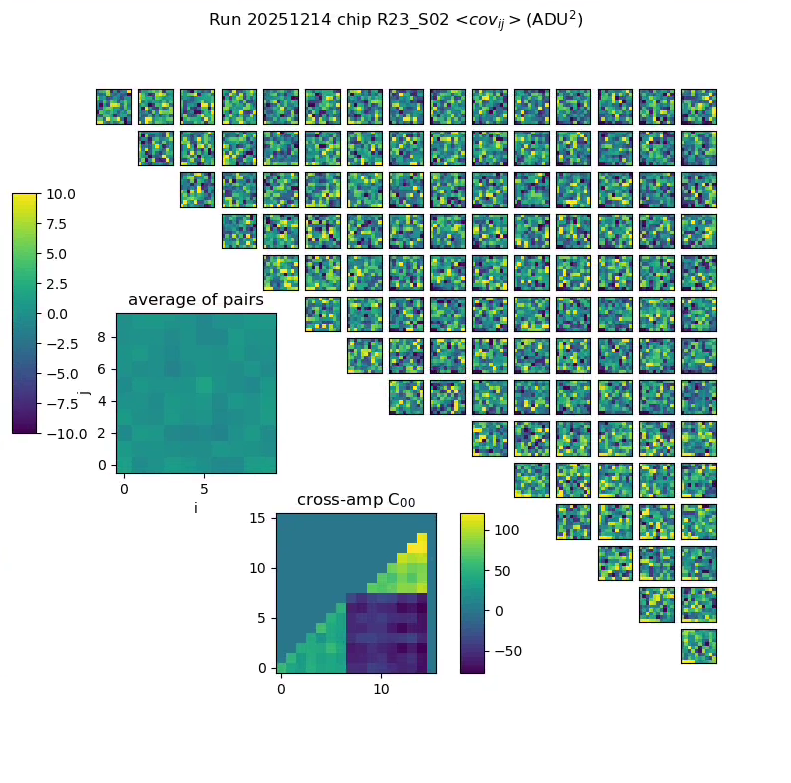
\includegraphics[width=0.48\linewidth]{sequencer/naturalfrequency/fig18b_covariance_grid_natural.png}
\caption{Covariances for all channel pairs of R23\_S02, excluding self-correlations, with the
average over pairs and the cross-amplifier \(C_{00}\) shown as insets. Left: run 20250715
(original). Right: run 20251214 (natural frequency). The checkerboard in the average of pairs
disappears (P.~Astier).}
\label{fig:nf-covariance-grid}
\end{centering}
\end{figure}

\begin{figure}[htbp]
\begin{centering}
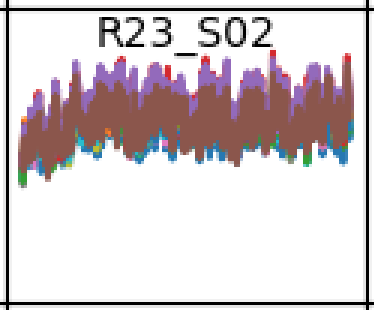
\includegraphics[width=0.3\linewidth]{sequencer/naturalfrequency/fig18c_relative_gain_r23s02_before.png}
\hspace{0.05\linewidth}
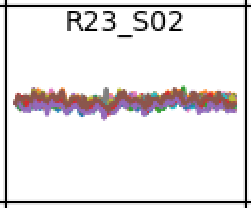
\includegraphics[width=0.3\linewidth]{sequencer/naturalfrequency/fig18d_relative_gain_r23s02_after.png}
\caption{Relative gain of R23\_S02 over the course of a run, on a vertical scale of \(\pm0.001\).
Left: original configuration. Right: with the natural frequency firmware.}
\label{fig:nf-relative-gain-insets}
\end{centering}
\end{figure}

\clearpage

\paragraph{Checkerboard in the PTC.}
The PTC products confirm the same result on the flats, through a completely different measurement.
Averaged over raft R22, the e2v noise matrix carries an unmistakable checkerboard in
\texttt{3s\_v1\_dp2\_v2}; with \texttt{3s\_v2} the pattern disappears and the colour scale shrinks
by an order of magnitude, from \(\pm0.08\) to \(\pm0.008\)
(Figure~\ref{fig:nf-ptc-noise-matrix-e2v}). The \(A\) matrix behaves the same way: the alternating
structure that was superimposed on the smooth brighter-fatter falloff is absent in the new data
(Figure~\ref{fig:nf-ptc-a-matrix-e2v}), which means the \(a_{ij}\) measurement is no longer
polluted. ITL, averaged over R02, shows the same improvement in the noise matrix at lower
amplitude (Figure~\ref{fig:nf-ptc-noise-matrix-itl}); the ITL \(A\) matrix was already free of the
pattern and is essentially unchanged, consistent with the checkerboard having been an e2v effect
from the start.

\begin{figure}[htbp]
\begin{centering}
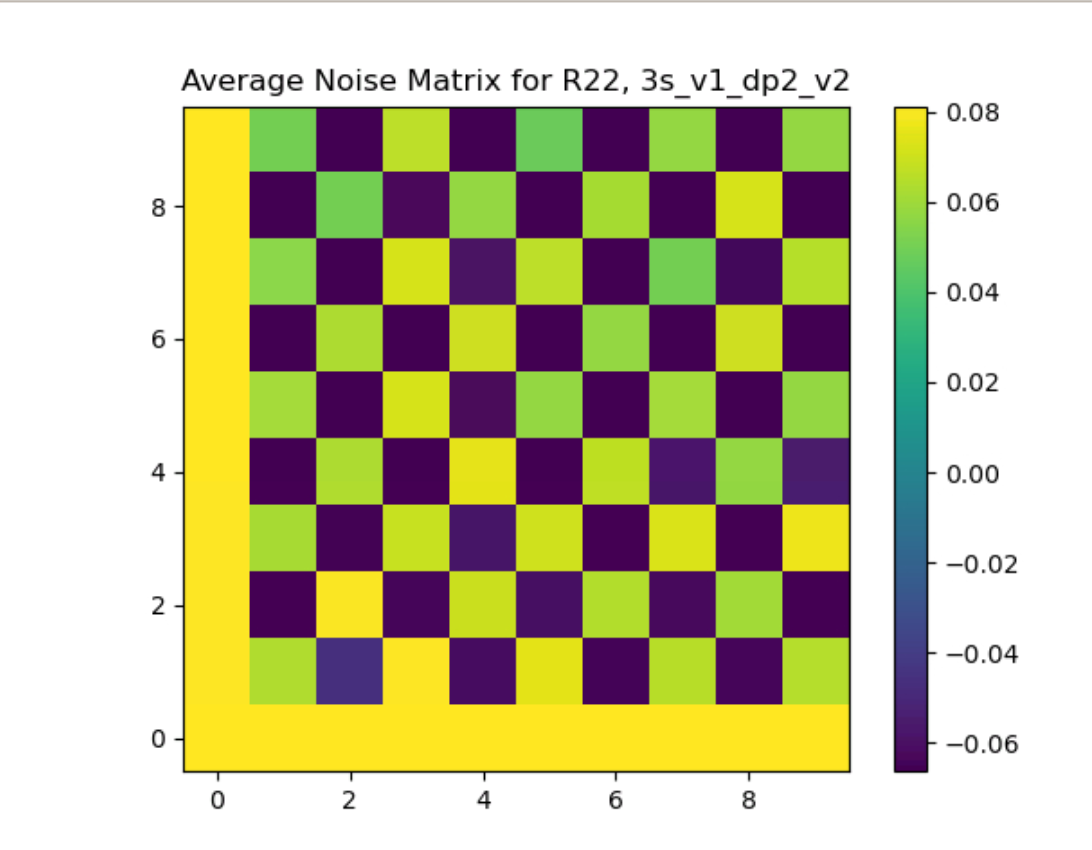
\includegraphics[width=0.48\linewidth]{sequencer/naturalfrequency/fig25a_ptc_noise_matrix_e2v_3sv1.png}
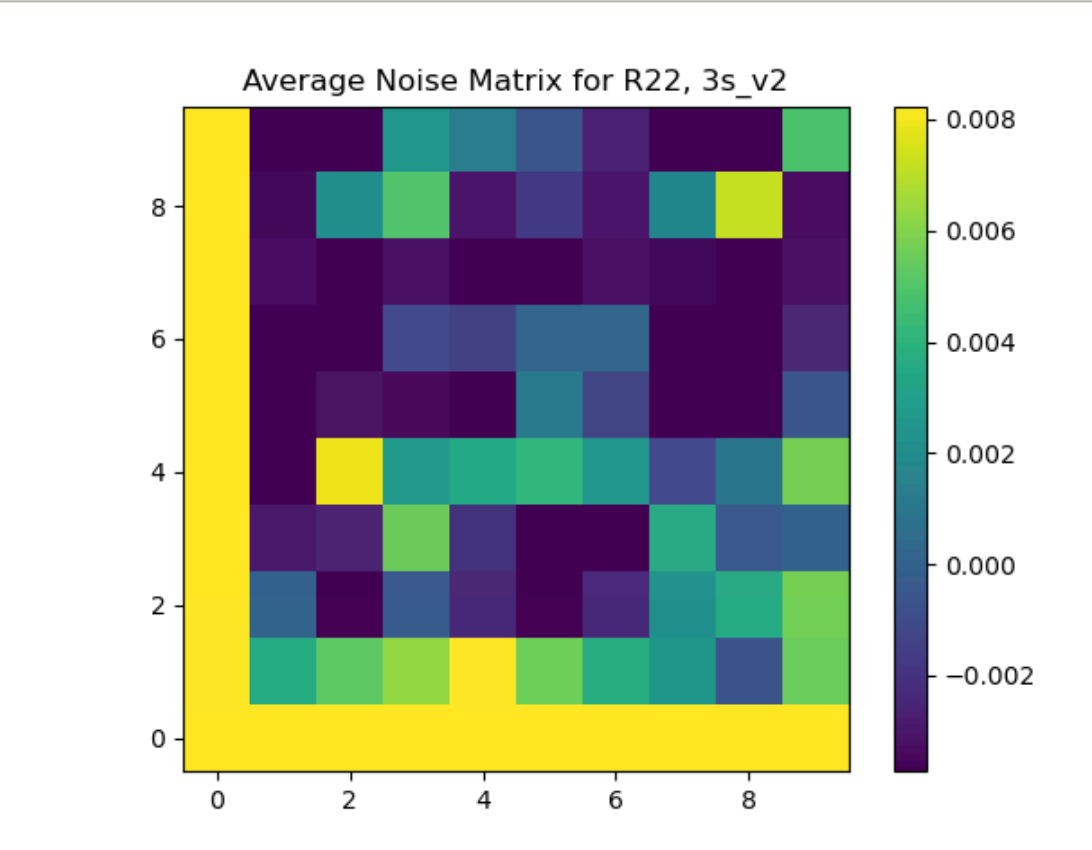
\includegraphics[width=0.48\linewidth]{sequencer/naturalfrequency/fig25b_ptc_noise_matrix_e2v_3sv2.png}
\caption{Average PTC noise matrix over raft R22 (e2v). Left: \texttt{3s\_v1\_dp2\_v2}. Right:
\texttt{3s\_v2}. Note that the colour scale differs by a factor of ten between the two panels
(E.~Rykoff).}
\label{fig:nf-ptc-noise-matrix-e2v}
\end{centering}
\end{figure}

\begin{figure}[htbp]
\begin{centering}
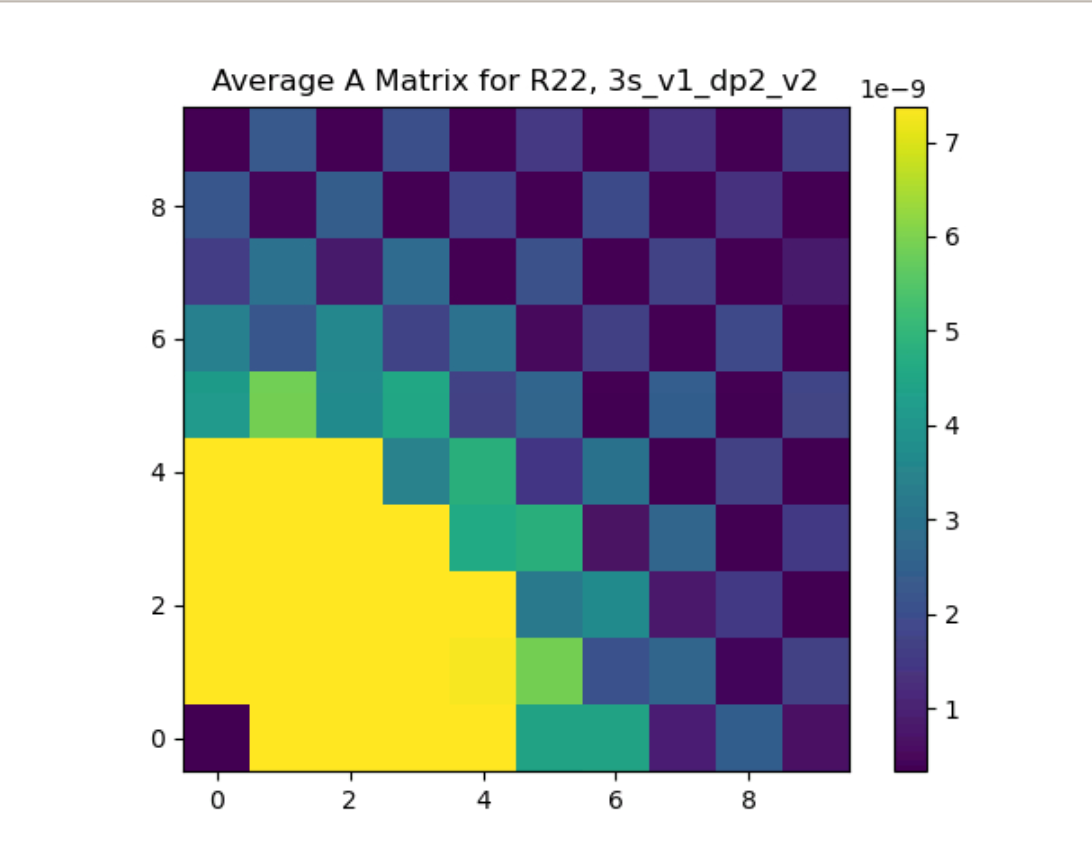
\includegraphics[width=0.48\linewidth]{sequencer/naturalfrequency/fig25c_ptc_a_matrix_e2v_3sv1.png}
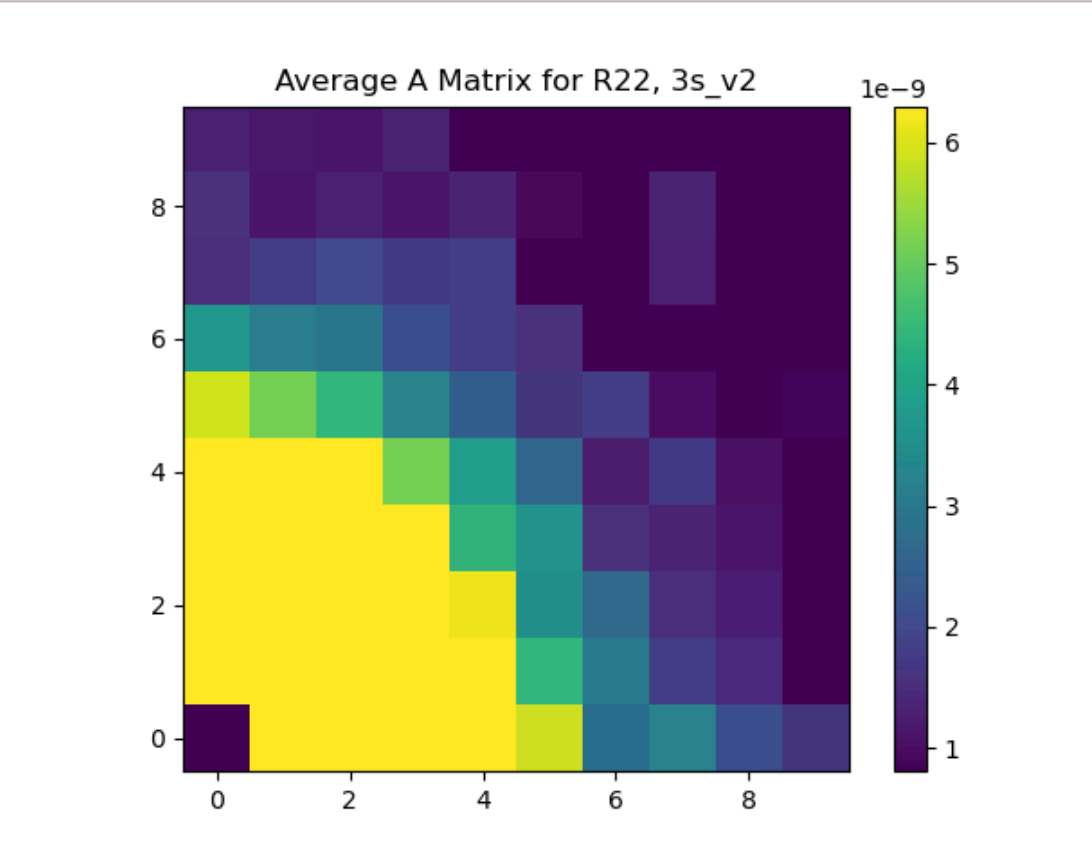
\includegraphics[width=0.48\linewidth]{sequencer/naturalfrequency/fig25d_ptc_a_matrix_e2v_3sv2.png}
\caption{Average \(A\) matrix over raft R22 (e2v). Left: \texttt{3s\_v1\_dp2\_v2}. Right:
\texttt{3s\_v2}. The checkerboard superimposed on the brighter-fatter falloff is gone
(E.~Rykoff).}
\label{fig:nf-ptc-a-matrix-e2v}
\end{centering}
\end{figure}

\begin{figure}[htbp]
\begin{centering}
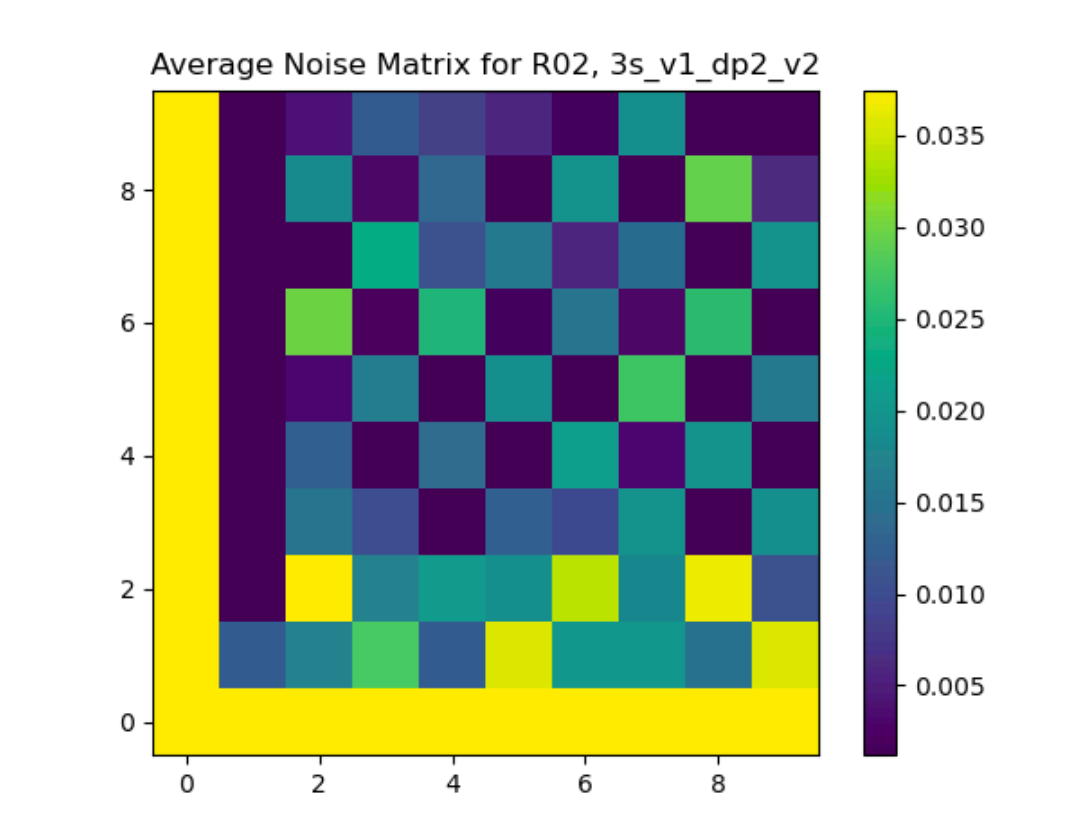
\includegraphics[width=0.48\linewidth]{sequencer/naturalfrequency/fig26a_ptc_noise_matrix_itl_3sv1.png}
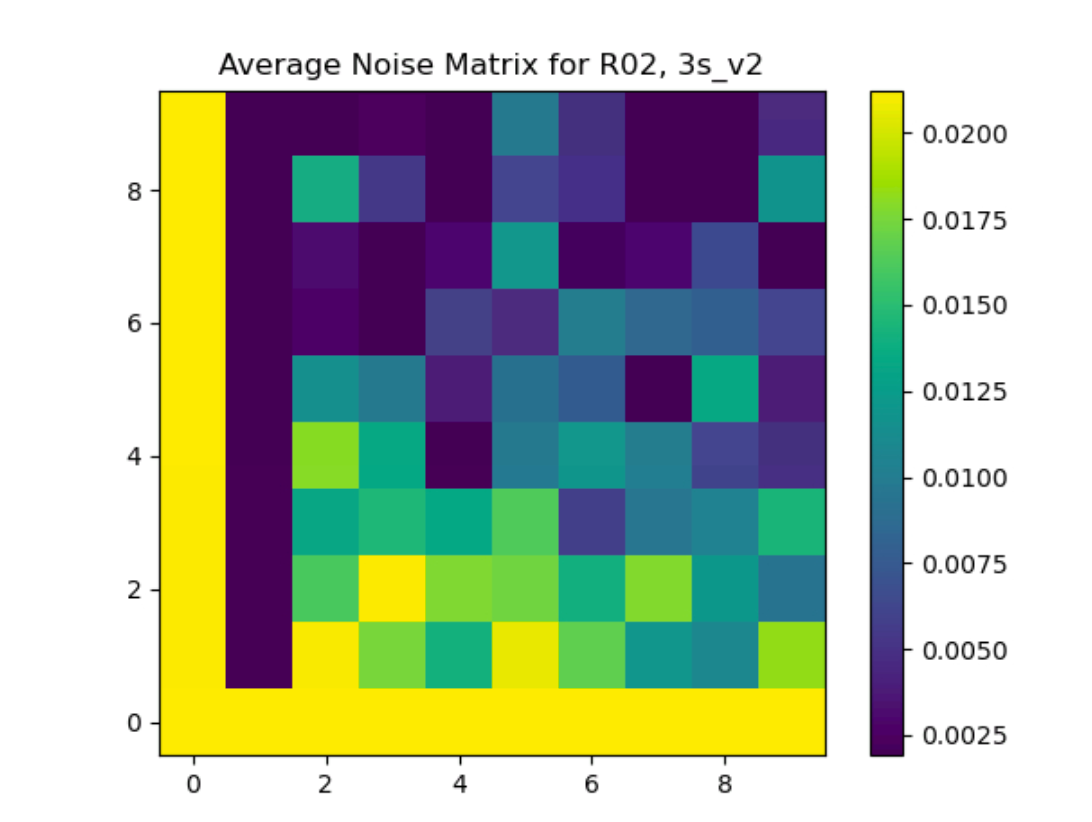
\includegraphics[width=0.48\linewidth]{sequencer/naturalfrequency/fig26b_ptc_noise_matrix_itl_3sv2.png}
\caption{Average PTC noise matrix over raft R02 (ITL). Left: \texttt{3s\_v1\_dp2\_v2}. Right:
\texttt{3s\_v2} (E.~Rykoff).}
\label{fig:nf-ptc-noise-matrix-itl}
\end{centering}
\end{figure}

\clearpage

%%
%% Results: linearity
%%
\paragraph{Linearity.}
The linearity solution improves as well, most visibly on the ITL detectors, where the structure
that the old solution left in the residuals is largely gone
(Figure~\ref{fig:nf-linearity-itl}). With \texttt{3s\_v1\_dp2\_v2} the residual fraction is spread
over roughly \(\pm1.5\times10^{-4}\) with visible wave-like structure across the full signal
range; with \texttt{3s\_v2} it collapses to a narrow band that tightens with signal, and the
usable range extends past \(10^5\)\,adu. Some ITL detectors improve only slightly (for example
detector 15), and the e2v detectors, which started in better shape, improve more modestly but
consistently (Figure~\ref{fig:nf-linearity-e2v}).

\begin{figure}[htbp]
\begin{centering}
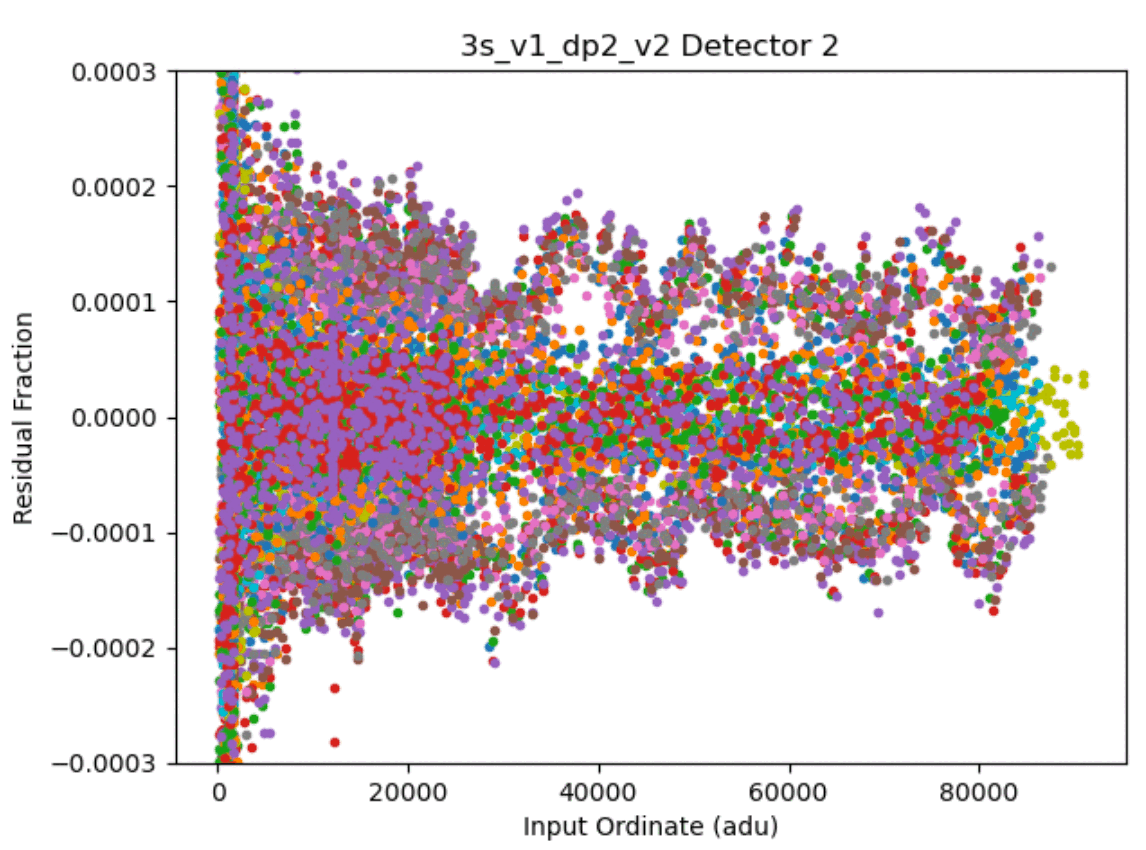
\includegraphics[width=0.48\linewidth]{sequencer/naturalfrequency/fig23a_linearity_itl_det2_3sv1.png}
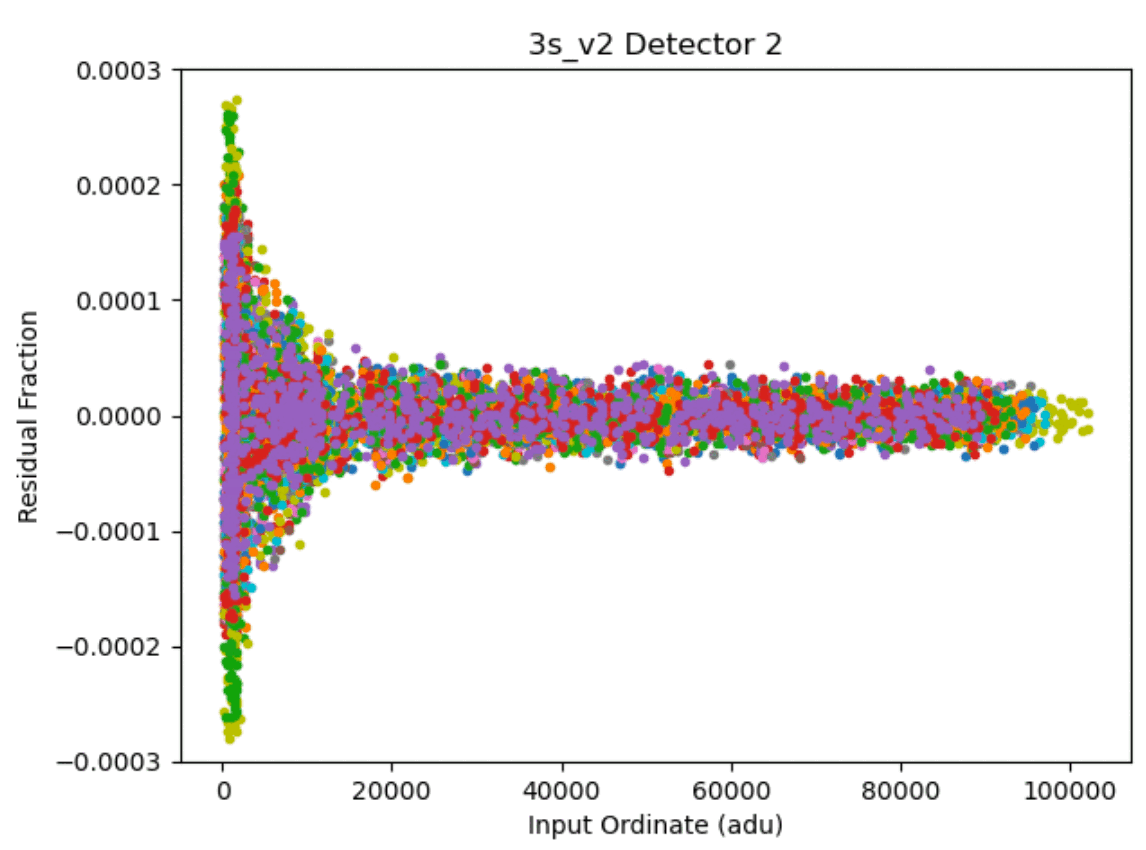
\includegraphics[width=0.48\linewidth]{sequencer/naturalfrequency/fig23b_linearity_itl_det2_3sv2.png}
\caption{Linearizer residual fraction against input ordinate for every amplifier of ITL detector
2. Left: \texttt{3s\_v1\_dp2\_v2}. Right: \texttt{3s\_v2}. The structure spread over
\(\pm1.5\times10^{-4}\) in the old solution collapses to a narrow band (E.~Rykoff).}
\label{fig:nf-linearity-itl}
\end{centering}
\end{figure}

\begin{figure}[htbp]
\begin{centering}
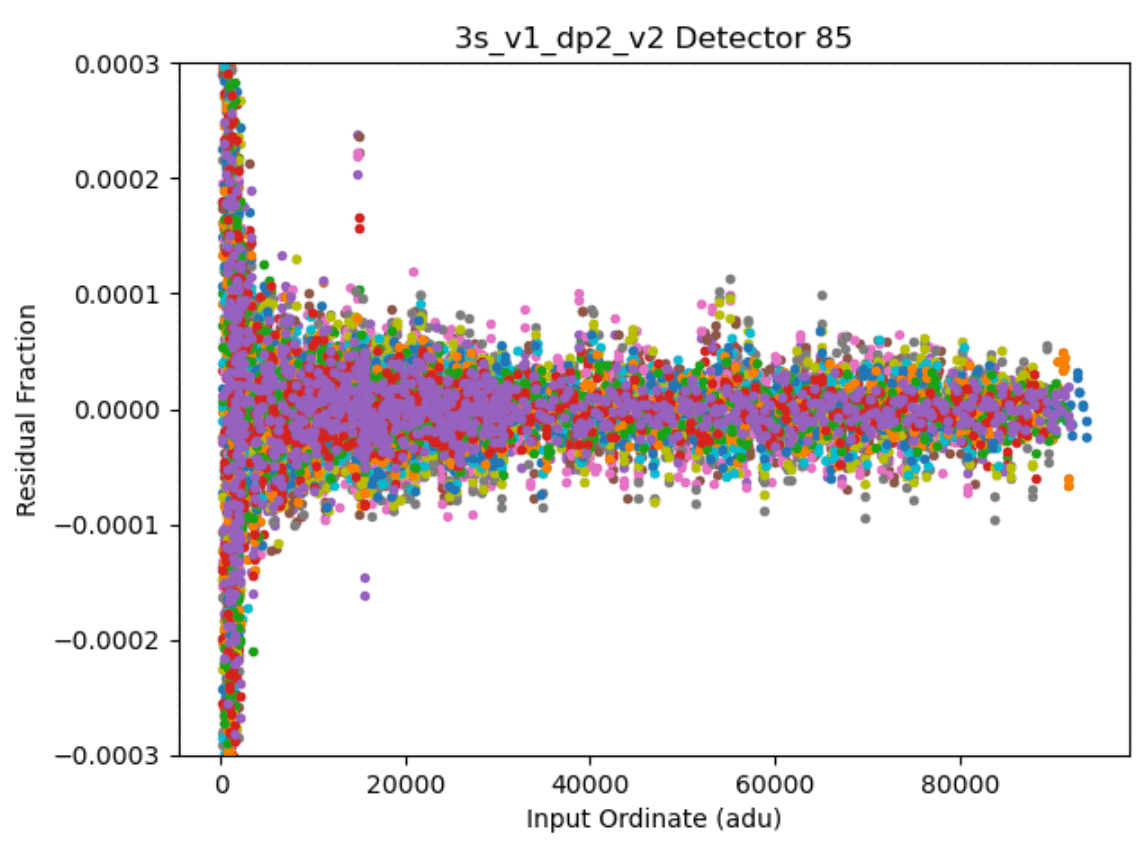
\includegraphics[width=0.48\linewidth]{sequencer/naturalfrequency/fig23c_linearity_e2v_det85_3sv1.png}
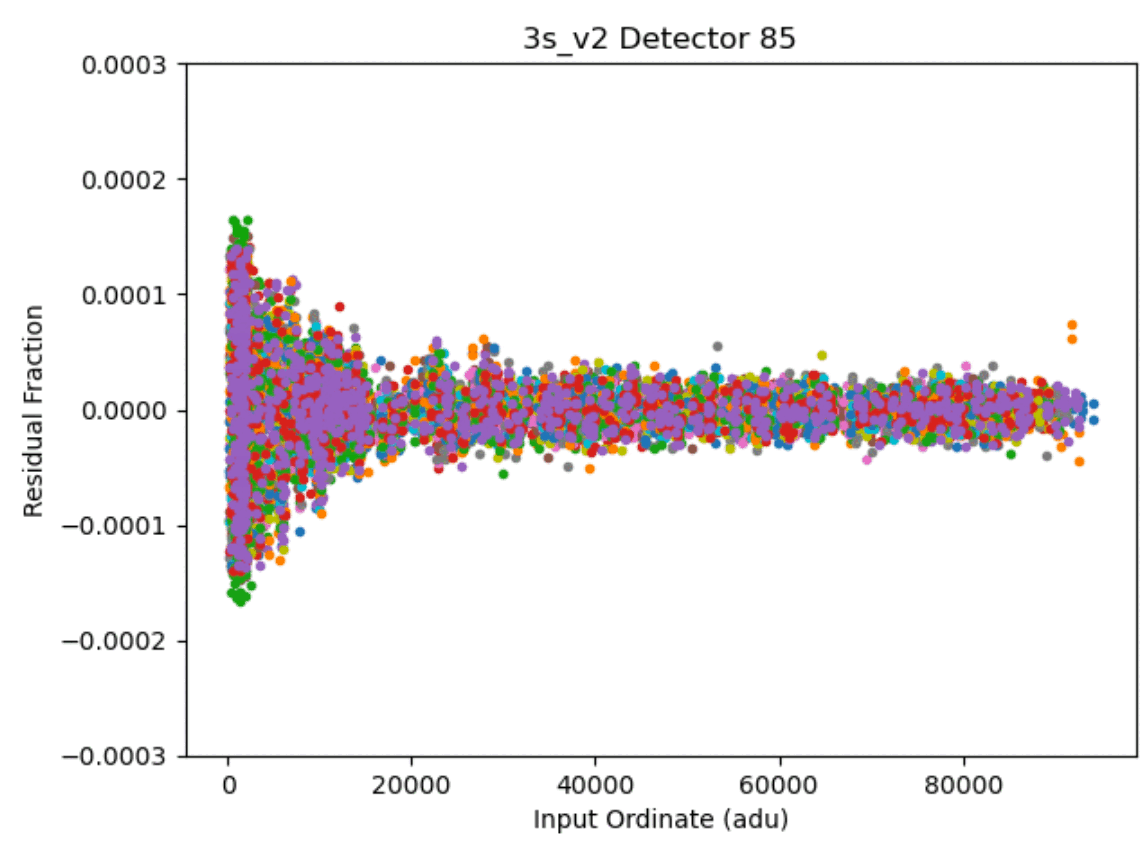
\includegraphics[width=0.48\linewidth]{sequencer/naturalfrequency/fig23d_linearity_e2v_det85_3sv2.png}
\caption{The same comparison for e2v detector 85, which was already in better shape. Left:
\texttt{3s\_v1\_dp2\_v2}. Right: \texttt{3s\_v2}.}
\label{fig:nf-linearity-e2v}
\end{centering}
\end{figure}

A handful of inner amplifiers still show structure in the \texttt{3s\_v2} residuals, and the
patterns differ from one another. On detector 41 (R22\_S12\_C14) the residuals appear correlated
with the overscan level, which is not typical of the focal plane. On detector 48
(R12\_S10\_C07) they correlate with time and possibly with the REB temperature, and on detector
152 (R33\_S22\_C03) with time alone, in both cases for a single amplifier on an otherwise
well-behaved detector. These are the linearity counterpart of the gain--temperature outliers noted
above.

The amplifiers at the edge of the focal plane show a residual that varies smoothly over the night
(Figure~\ref{fig:nf-edge-illumination}). The same or similar patterns appear on all partly
vignetted and nearly-partly-vignetted detectors, for example detector 178 (R42\_S21), while the
inner amplifiers and detectors show nothing of the kind. Variable illumination at the edges is the
natural explanation, and it accounts for the edge outliers in the flat-field gain stability above.

\begin{figure}[htbp]
\begin{centering}
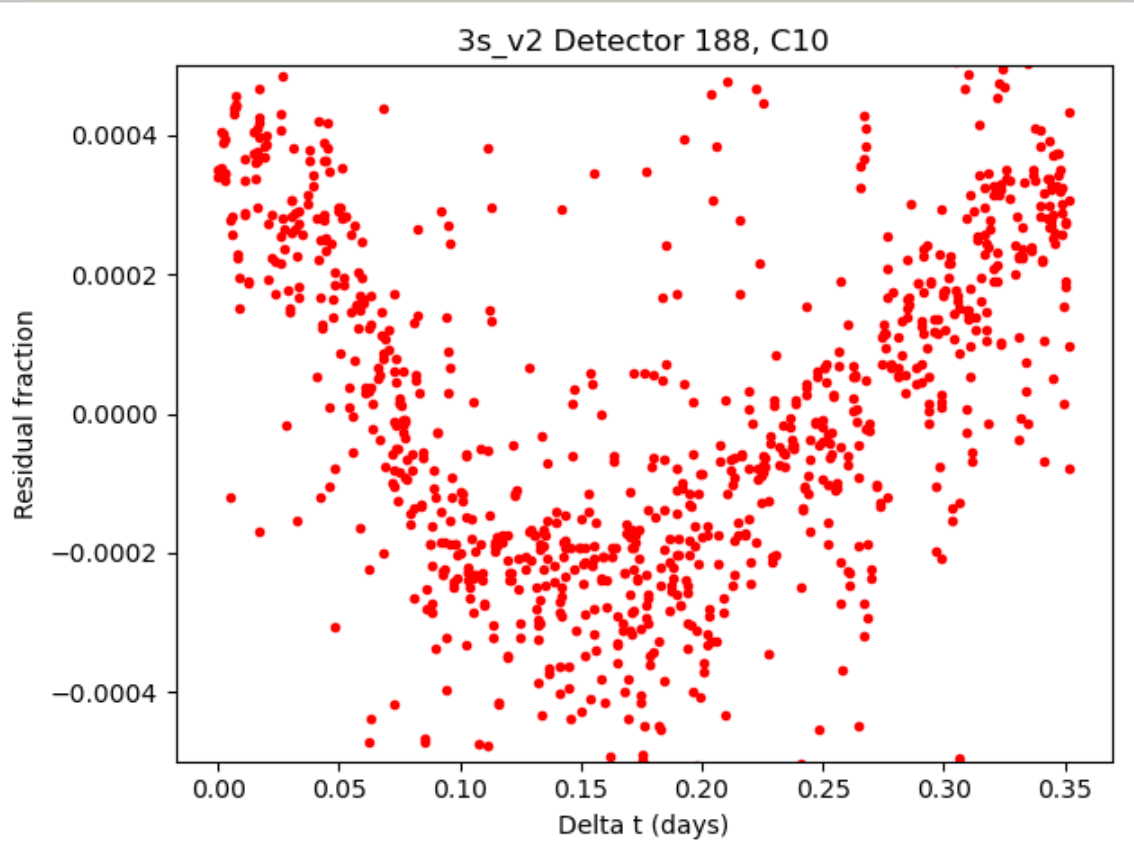
\includegraphics[width=0.6\textwidth]{sequencer/naturalfrequency/fig24_edge_illumination_det188.png}
\caption{Absolute linearizer residual fraction against elapsed time for detector 188
(R43\_S22), amplifier C10, with the \texttt{3s\_v2} data. The smooth variation over the night is
seen on the partly vignetted detectors only (E.~Rykoff).}
\label{fig:nf-edge-illumination}
\end{centering}
\end{figure}

\paragraph{PTC turnoff.}
The PTC turnoffs, expressed in electrons, are broadly consistent between the two configurations,
with a set of outliers and a locus of e2v turnoffs that moved up
(Figure~\ref{fig:nf-ptc-turnoff}); both are still being followed up.

\begin{figure}[htbp]
\begin{centering}
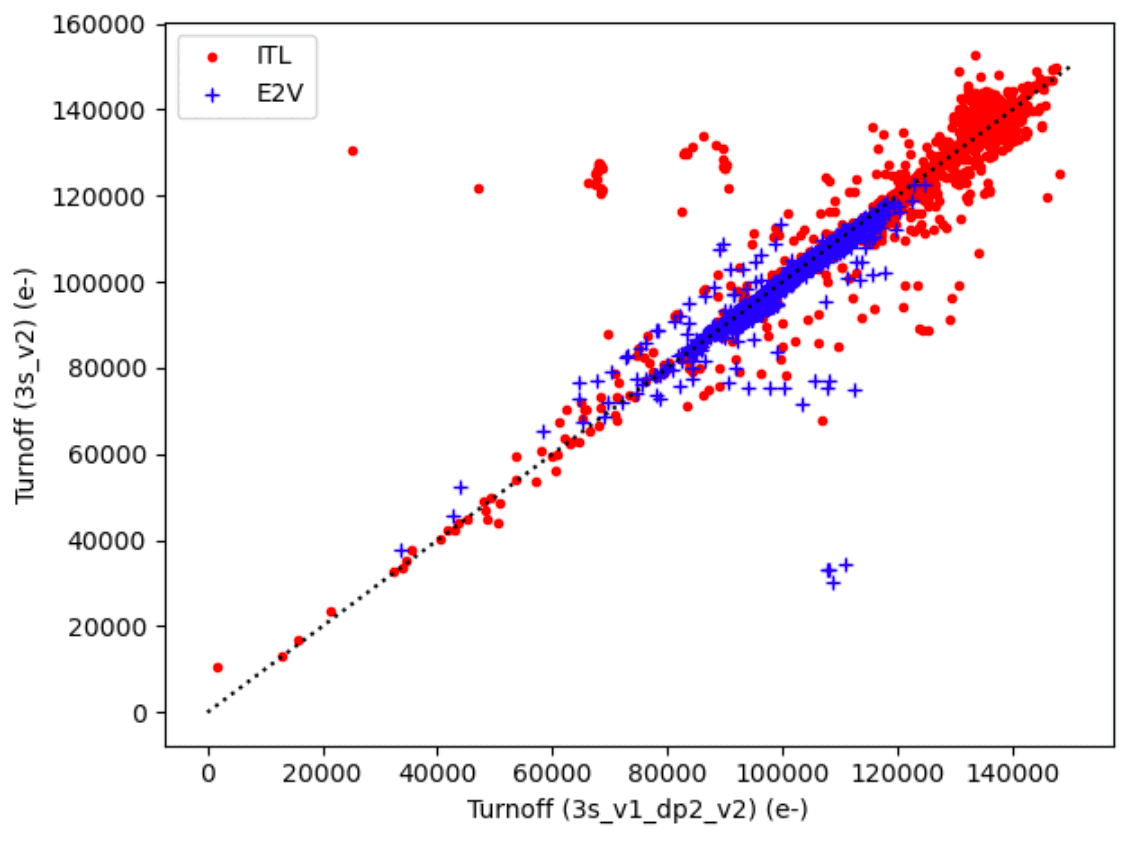
\includegraphics[width=0.55\textwidth]{sequencer/naturalfrequency/fig27c_turnoff_comparison.png}
\caption{Per-amplifier PTC turnoff in electrons, \texttt{3s\_v1\_dp2\_v2} against
\texttt{3s\_v2} (E.~Rykoff).}
\label{fig:nf-ptc-turnoff}
\end{centering}
\end{figure}

\clearpage

%%
%% Results: science images
%%
\paragraph{Science images.}
Science images were taken with the natural frequency firmware on 3 January 2026 (for example
exposures 655 and 657); two examples are shown in Figure~\ref{fig:nf-science-images}. The expected
gap in illumination between ITL and e2v sensors, caused by the small gain change, is visible, as
is a small crosstalk residue. Both are expected, since no calibration products were regenerated
for these frames. No other issue was found.

\begin{figure}[htbp]
\begin{centering}
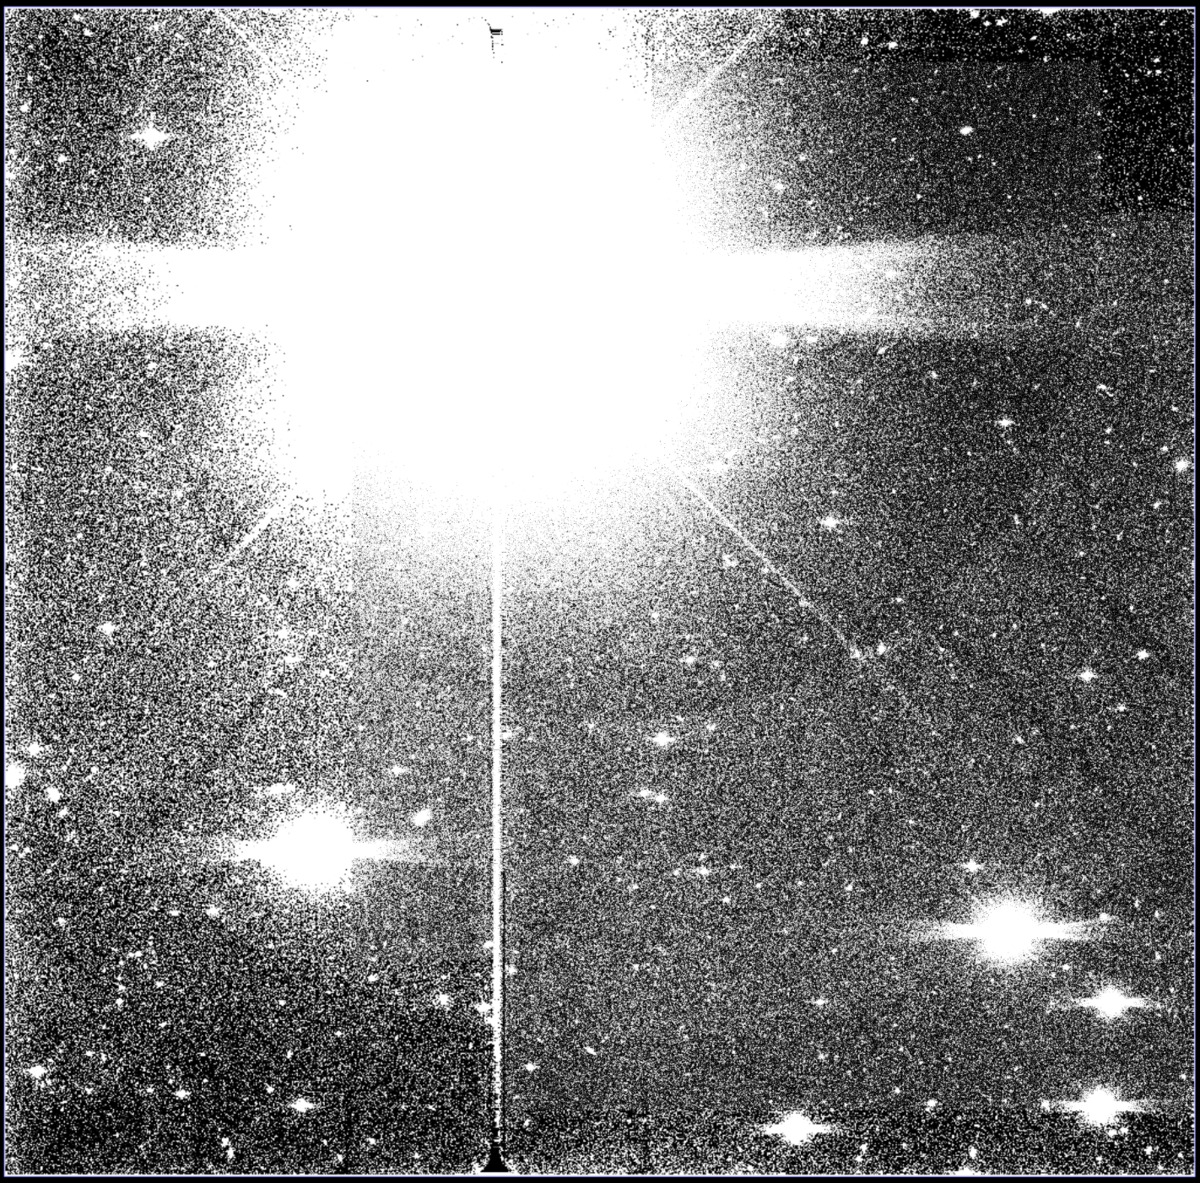
\includegraphics[width=0.45\linewidth]{sequencer/naturalfrequency/fig19a_science_image_left.jpg}
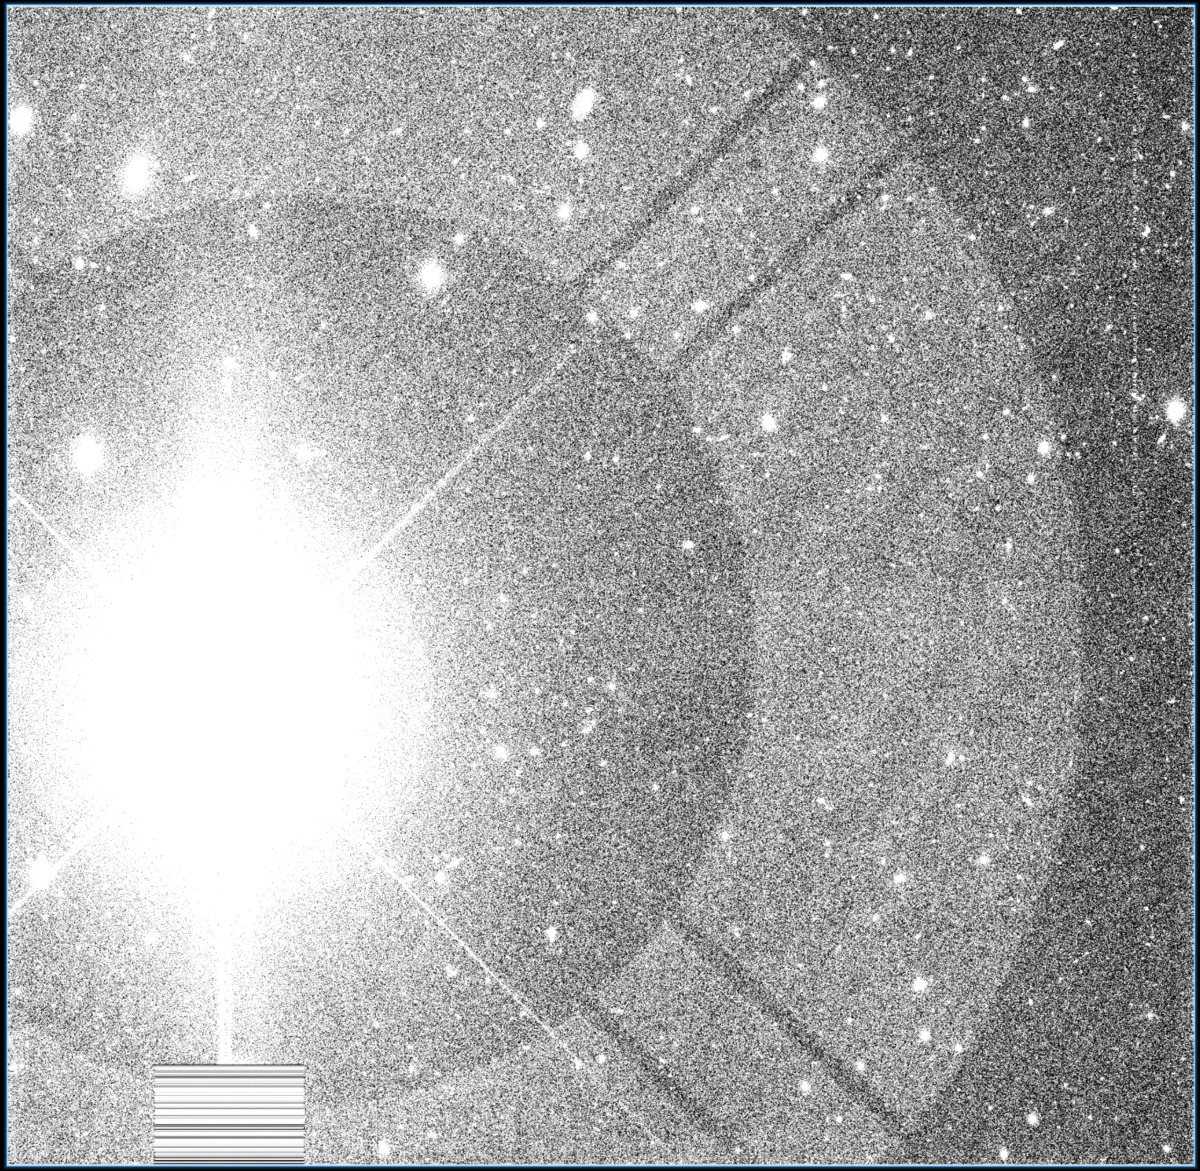
\includegraphics[width=0.45\linewidth]{sequencer/naturalfrequency/fig19b_science_image_right.jpg}
\caption{Two science images acquired with the natural frequency firmware on 3 January 2026,
around a saturated star. The residual crosstalk and the illumination step between vendors are
visible at low level.}
\label{fig:nf-science-images}
\end{centering}
\end{figure}

\clearpage

%%
%% LATISS / WREB and the wavefront sensors
%%
\paragraph{LATISS testing (WREB).}
The WREB behaves differently. The noise measurement in the noise--bias plane is noisier than for
the science rafts (Figure~\ref{fig:nf-wreb-noise-bias}), and print-through was identified as the
cause: a section of the serial overscan shows the print-through structure directly
(Figure~\ref{fig:nf-wreb-overscan}). Disabling the ASPIC temperature read made the print-through
go away. The pattern in the covariance, however, still exists in a different form, and is present
whether or not the science rafts are running the natural frequency firmware
(Figure~\ref{fig:nf-wreb-covariance}).

\begin{figure}[htbp]
\begin{centering}
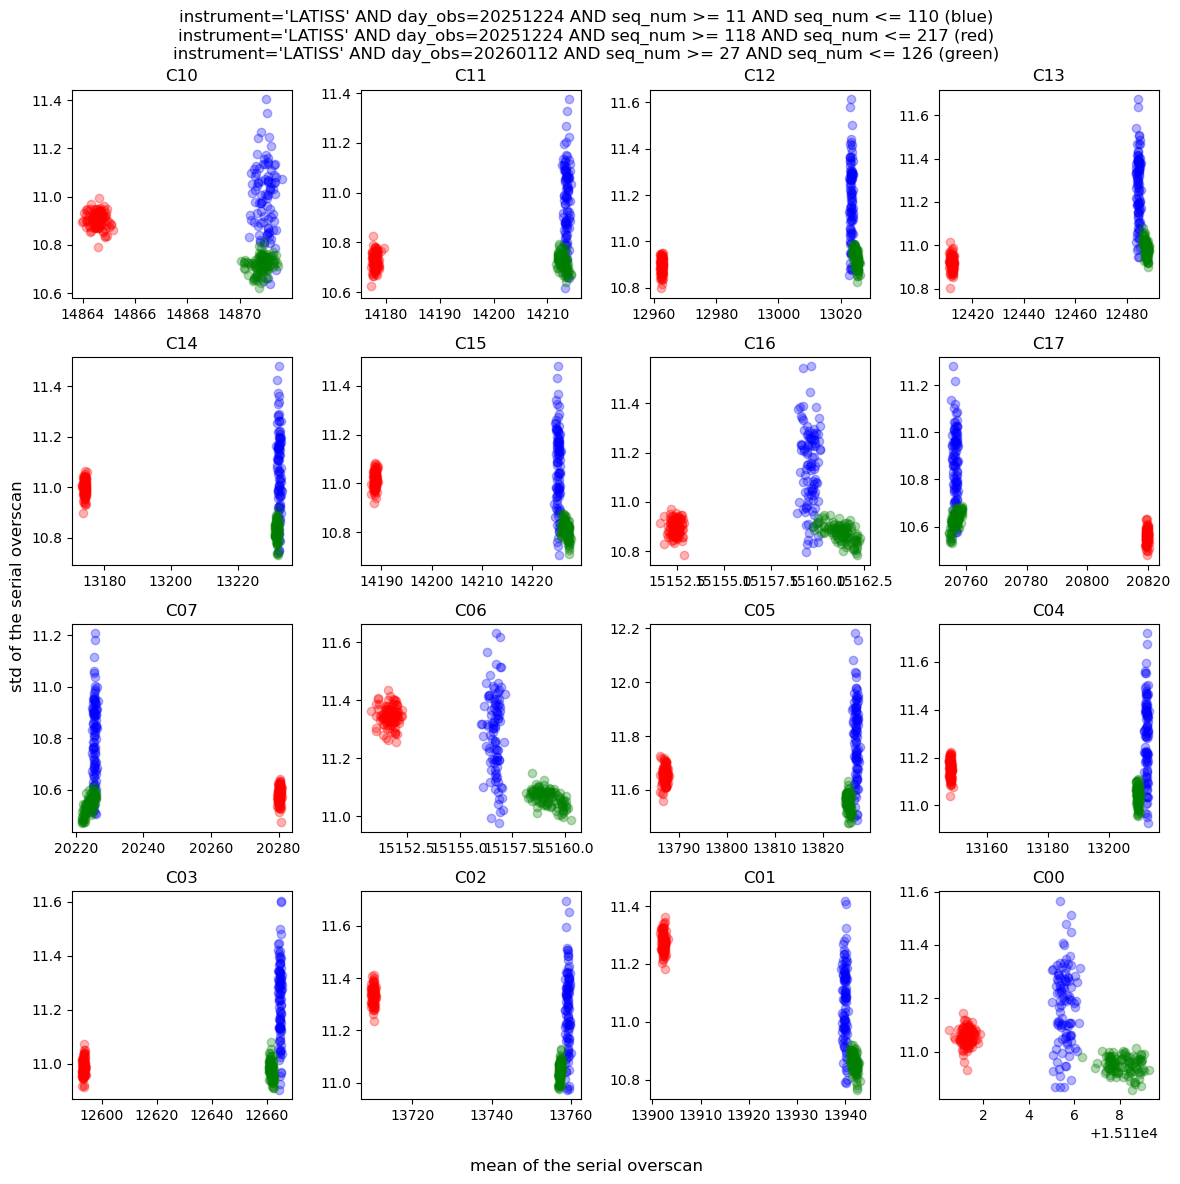
\includegraphics[width=0.8\textwidth]{sequencer/naturalfrequency/fig20a_wreb_noise_bias_scatter.png}
\caption{Standard deviation versus mean of the serial overscan for each amplifier of LATISS, for
three acquisitions: 20251224 sequence numbers 11--110 (blue), 20251224 sequence numbers 118--217
(red) and 20260112 sequence numbers 27--126 (green).}
\label{fig:nf-wreb-noise-bias}
\end{centering}
\end{figure}

\begin{figure}[htbp]
\begin{centering}
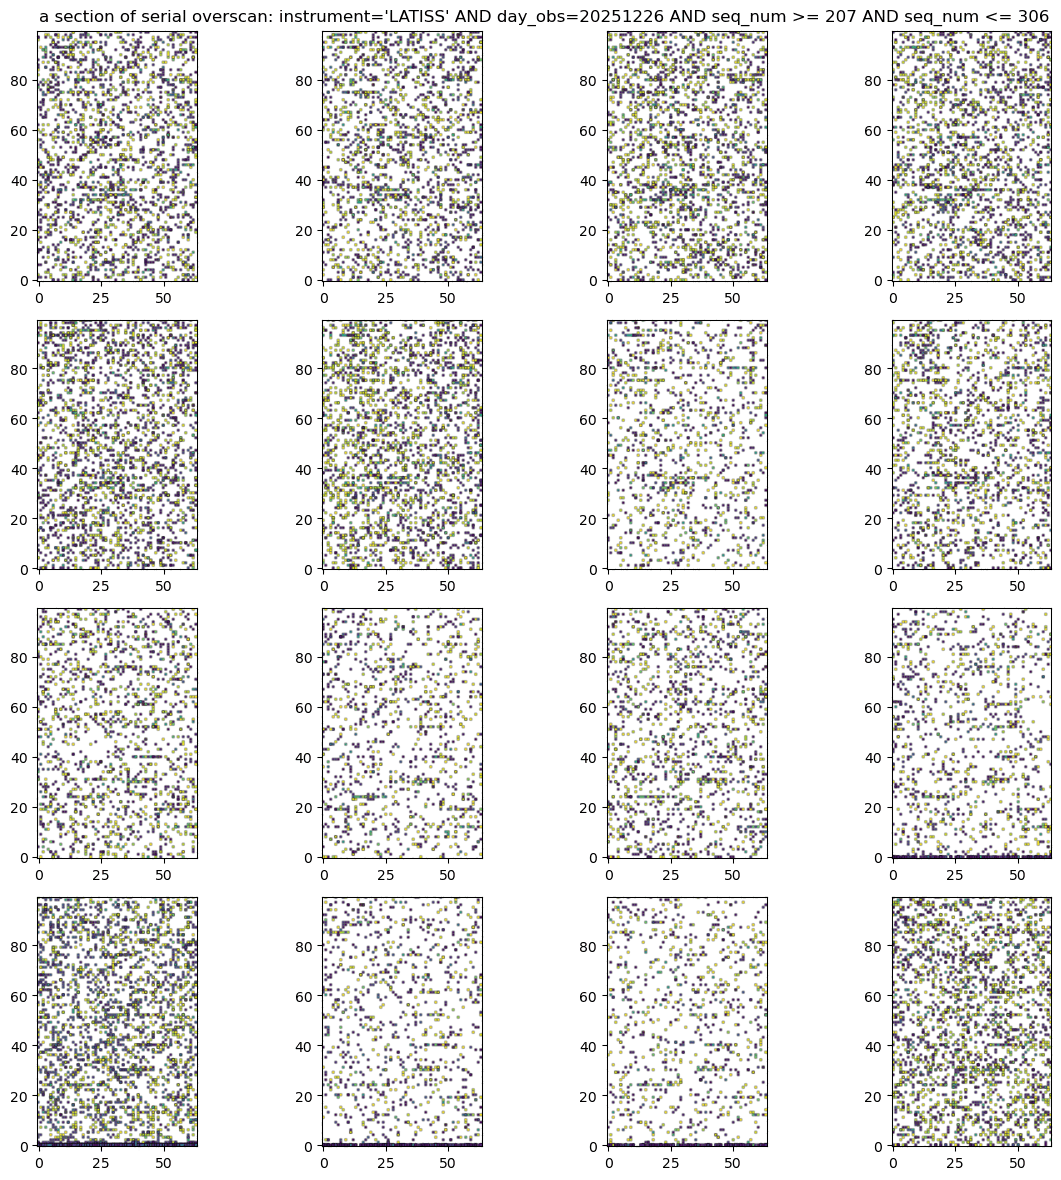
\includegraphics[width=0.7\textwidth]{sequencer/naturalfrequency/fig20b_wreb_serial_overscan_section.png}
\caption{A section of the serial overscan for LATISS, 20251226, sequence numbers 207--306,
showing the print-through structure.}
\label{fig:nf-wreb-overscan}
\end{centering}
\end{figure}

\begin{figure}[htbp]
\begin{centering}
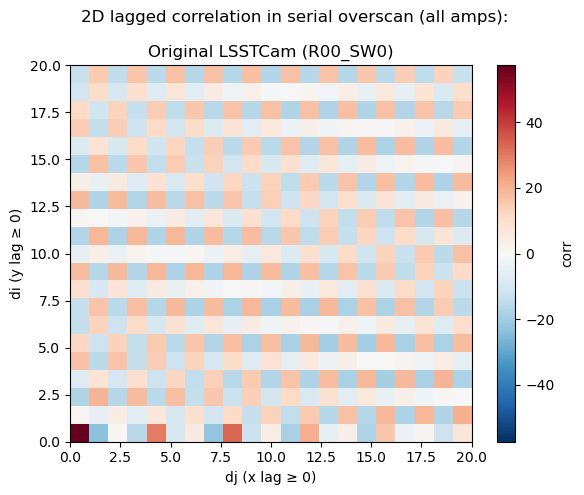
\includegraphics[width=0.48\linewidth]{sequencer/naturalfrequency/fig20c_wreb_checkerboard_original.png}
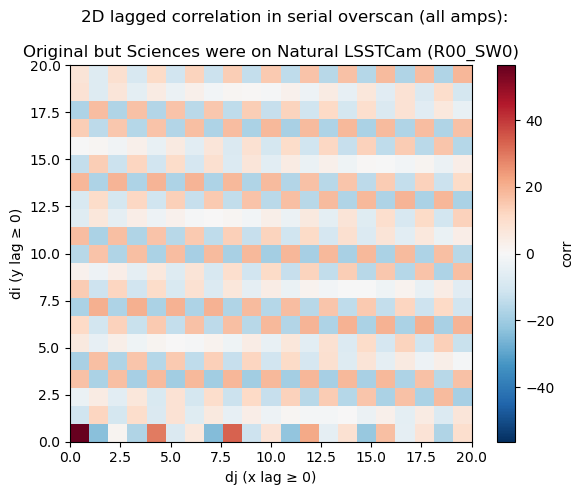
\includegraphics[width=0.48\linewidth]{sequencer/naturalfrequency/fig20d_wreb_checkerboard_original_natural_science.png}
\caption{Two-dimensional lagged correlation in the serial overscan for R00\_SW0. Left: original
configuration. Right: original WREB configuration while the science rafts were running the
natural frequency firmware. The pattern persists in both.}
\label{fig:nf-wreb-covariance}
\end{centering}
\end{figure}

The PTC products flag a wavefront problem of their own: one amplifier, R40\_SW1\_C13, produces an
\(A\) matrix in the new run that is clearly wrong, showing alternating rows that saturate both
ends of a colour scale two orders of magnitude larger than expected, where the old run gave the
smooth brighter-fatter structure (Figure~\ref{fig:nf-wf-amatrix}). Whether this is the same
underlying WREB behaviour seen in the PTC is not yet established.

\begin{figure}[htbp]
\begin{centering}
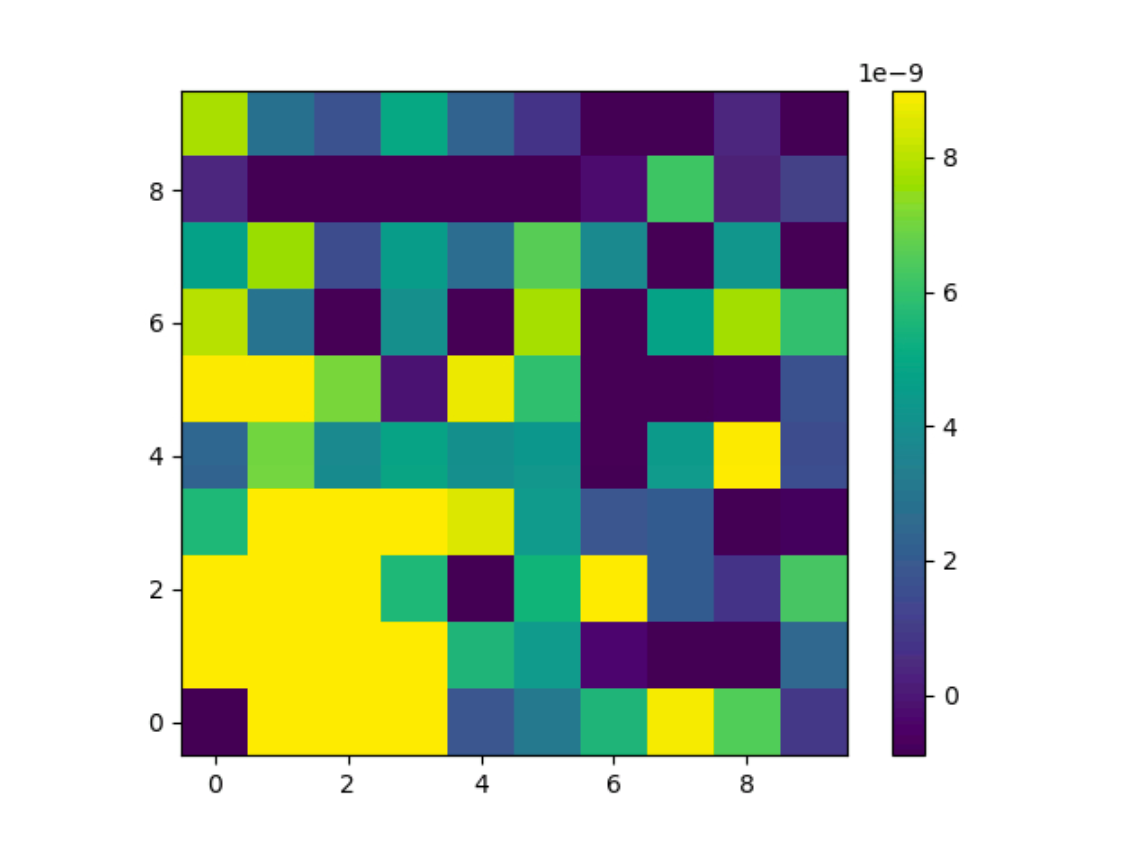
\includegraphics[width=0.48\linewidth]{sequencer/naturalfrequency/fig28a_wf_amatrix_old.png}
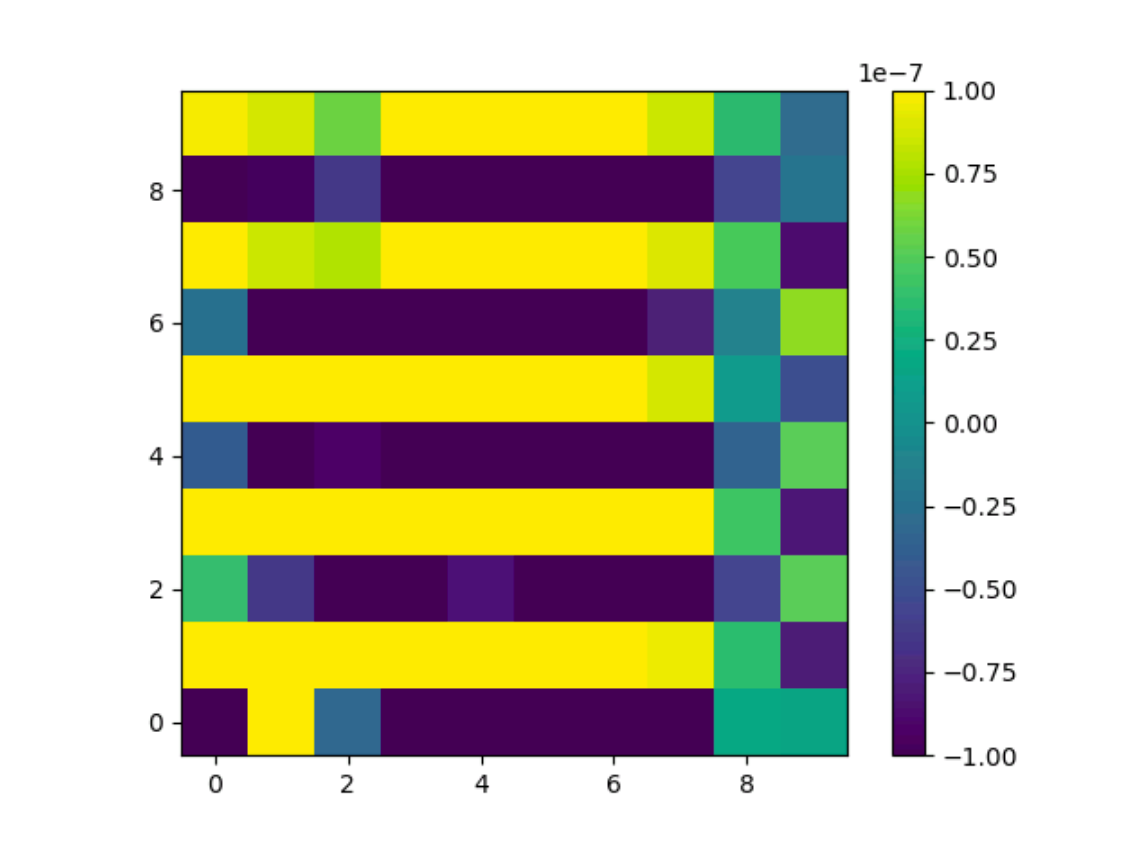
\includegraphics[width=0.48\linewidth]{sequencer/naturalfrequency/fig28b_wf_amatrix_new.png}
\caption{\(A\) matrix for R40\_SW1\_C13. Left: old run, as expected. Right: new run, with
alternating rows and a colour scale two orders of magnitude larger (E.~Rykoff).}
\label{fig:nf-wf-amatrix}
\end{centering}
\end{figure}

\clearpage

%%
%% Wavefront sensors / scan mode
%%
\paragraph{Understanding the wavefront sensors.}
Scan mode is the natural tool for understanding the underlying issue, since it resolves the
signal within the sequencer time slots. The scan-mode data taken on R00\_SW0 in run 13108
(Figure~\ref{fig:nf-scanmode}) show a wild signal after the RST/CL toggling, wiggles in the first
ramp, and an increase of the noise for a longer ramp time. These acquisitions have not been
repeated since November 2023. Progress requires getting TS8 running and testing there, and then
stepping to LATISS and LSSTCam.

\begin{figure}[htbp]
\begin{centering}
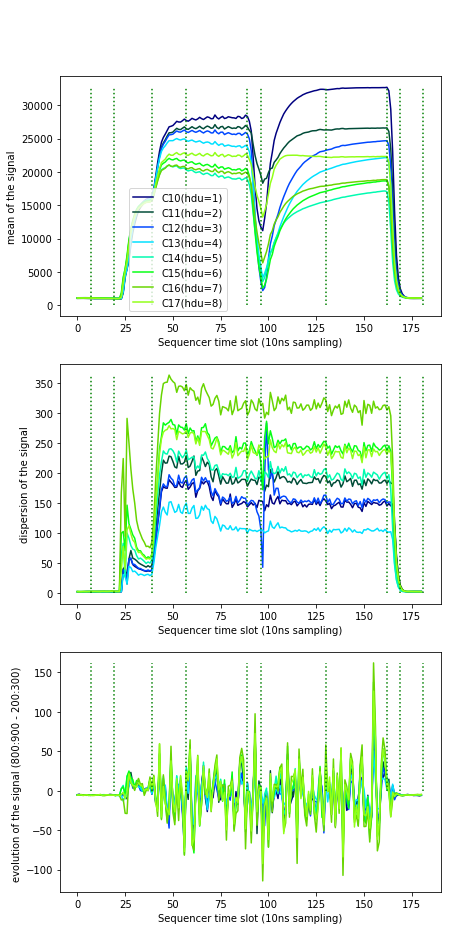
\includegraphics[width=0.5\textwidth]{sequencer/naturalfrequency/fig21_scanmode_r00_sw0.png}
\caption{Scan-mode data for R00\_SW0, run 13108, sampled every 10\,ns of the sequencer. Top: mean
of the signal for the eight channels. Middle: dispersion of the signal. Bottom: evolution of the
signal between scans 800--900 and 200--300. Dotted lines mark the sequencer transitions.}
\label{fig:nf-scanmode}
\end{centering}
\end{figure}

%%
%% Summary
%%
\paragraph{Summary.}
Two independent campaigns, one on bias and flat frames and one on the PTC and linearizer products,
agree on what the natural frequency firmware and the \texttt{3s-v2} sequencer accomplished. The
bias multimodality is removed, both in the noise--bias plane and in the row profiles, and the gain
variation is now better than \(\mathcal{O}(10^{-4})\); the PTC gains and read noise confirm this
amplifier by amplifier, with the noise improving markedly on the e2v channels that had carried
the excess variance. Since the behaviour is unchanged across REB resets, the conversion of the
clocks from 6.4\,ns to 10\,ns on the REB, rather than the REB synchronization itself, appears to
be the source of the inconsistency.

The checkerboard is gone in the overscan lagged correlations, in the cross-amplifier covariances,
and in the PTC noise and \(A\) matrices alike, so the \(a_{ij}\) measurement is no longer
polluted. It is likely cured by the even--odd change rather than by the natural frequency, which
implies that a small difference remains between the members of a pair of clocks; the sequencer
carrying both changes is the one adopted in production as \texttt{3s-v2}. The linearity solution
improves at the same time, most strongly for ITL. No major issue was observed in the science
images taken with the new firmware.

What remains is consistent between the two campaigns: residual patterns on the vignetted edge
detectors, which both attribute to variable illumination, and a small number of amplifiers whose
gain or linearity residual correlates with time and temperature. The PTC turnoff outliers and the
locus of e2v turnoffs that moved up are still being followed up. The WREB remains a mystery, with
a print-through cured by disabling the ASPIC temperature read but a covariance pattern that
persists, and a wavefront amplifier whose \(A\) matrix is clearly wrong in the new run. The GREB
is next after it. Scan-mode measurements on the focal plane and on LATISS, and the 0/1/2D bias
analysis of T.~Guillemin, are the natural next steps.

\clearpage
